%TEX program = xelatex
%表示用xelatex编译文件
\documentclass[a4paper]{ctexart}
\usepackage{ulem}
\usepackage{array}
\usepackage{tabularx}
\usepackage{indentfirst} 
\setlength{\parindent}{2em}
\usepackage{booktabs}
\usepackage{multirow}
\usepackage{makecell}
\usepackage{graphicx}
\usepackage{subfig}
\usepackage{amsmath,amsfonts,amssymb,amsthm}
\usepackage{amsbsy}
\usepackage{latexsym}
\usepackage{float}
\DeclareMathOperator{\argh}{argh} 
\DeclareMathOperator*{\nut}{Nut}
\usepackage{yhmath}
\usepackage{eucal,mathrsfs}
\usepackage[T1]{fontenc}
\usepackage{txfonts}
\usepackage{fontspec}
%\setsansfont[BoldFont={Arial Bold}, ItalicFont={Arial Italic}]{Arial}

\begin{document}
    \title{标题页}
    \author{Ryan\thanks{注脚}%
        \and Fan\thanks{注脚}%
        }
    \date{\today}
    \maketitle
    \abstract
    一般用于紧跟\textbackslash maketitle 命令之后介绍文档的摘要\par
    中文\LaTeX{}排版。
    \section{用\LaTeX 排版文字}
    {}分段\\换行\textbackslash\textbackslash\par
    冒号``please press the `x' key.''\par
    连字符-用来组成复合词,\\%
    短破折号--用来连接数字表示范围,\\%
    长破折号---用来连接单词\par
    省略号\dots{}和\ldots\par
    波浪号~\par
    强调\underline{文字,但是无法换行,}%
    \uline{ulem 宏包解决了这一问题,它提供的 uline 命令能够轻松生成自动换行的下划线。}%
    \emph{emph 命令用来将文字变为斜体以示强调。%
        \emph{如果在本身已经用 emph 命令强调的文字内部嵌套使用 emph 命令,}%
        内部则使用直立体文字。%
        }\par
    在合适的位置插入一个不会断行的空格Fig.~1, Ryan~Fan\par
    断行\\[15pt]可以带可选参数 $\langle length\rangle$,用于在换行处向下增加垂直间距%
    \newline{}或者newline命令,不用带参数\par
    \newpage 断页,在在双栏排版中只起到另起一栏的作用\par
    断词 I think this is: supercalifragil\-isticexpialidocious. %
    And I think this is: supercalifragilisticexpialidocious.\par
    \newpage
    \tableofcontents
    \newpage
    \section[目录和页眉页脚]{章节}
    \subsection{子章节}
    \subsubsection{子子章节}
    \paragraph{段落}
    \subparagraph{子段落}
    \section*{标题不带编号}
    \addcontentsline{toc}{section}{标题不带编号}
    \part{分块}
    \section{交叉引用}
    A reference to this subsection\label{sec:this} looks like: %
    ``see section~\ref{sec:this} on page~\pageref{sec:this}.''
    \section{脚注和边注}
    “天地玄黄,宇宙洪荒。日月盈昃,辰宿列张。”\footnote{出自《千字文》。}\par
    \begin{tabular}{l}
        \hline
        有些情况下(比如在表格环境、各种盒子\\
        内)使用 footnote 并不能正确生成脚\\
        注。我们以分两步进行,先使用 \\
        footnotemark 为脚注计数,再在合适\\
        的位置用 footnotetext 生成脚注。\footnotemark\\
        \hline
    \end{tabular}
    \footnotetext{出自《千字文》。}
    \marginpar{\footnotesize 边注较窄,不要写过多文字,最好设置较小的字号。}
    \section{特殊环境}
    \subsection{列表}
    有序列表
    \begin{enumerate}
        \item An item.
        \begin{enumerate}
            \item A nested item.\label{itref}
            \item[*] A starred item.
        \end{enumerate}
        \item Reference(\ref{itref}).
    \end{enumerate}
    无序列表
    \begin{itemize}
        \item An item.
        \begin{itemize}
            \item A nested item.
            \item[+] A `plus' item. + A ‘plus’ item.
            \item Another item. – Another item.
        \end{itemize}
        \item Go back to upper level.
    \end{itemize}
    关键字环境
    \begin{description}
        \item[Enumerate] Numbered list.
        \item[Itemize] Non-numbered list.
    \end{description}
    重定义无序列表的符号
    \renewcommand{\labelitemi}{\dag}
    \renewcommand{\labelitemii}{\ddag}
    \begin{itemize}
        \item First item
        \begin{itemize} 
            \item Subitem
            \item Subitem
        \end{itemize}
        \item Second item
    \end{itemize}
    重定义有序列表的符号
    \renewcommand{\labelenumi}{\Alph{enumi}>}
    \begin{enumerate}
        \item First item
        \item Second item
    \end{enumerate}
    \subsection{对齐环境}
    center、flushleft 和 flushright 环境分别用于生成%
    居中、左对齐和右对齐的文本环境。
    \begin{center}
        Centered text using a
        \verb|center| environment.
    \end{center}
    \begin{flushleft}
        Left-aligned text using a
        \verb|flushleft| environment.
    \end{flushleft}
    \begin{flushright}
        Right-aligned text using a
        \verb|flushright| environment.
    \end{flushright}
    还可以用以下命令直接改变文字的对齐方式:
    \centering
    Centered text paragraph.\par
    \raggedright
    Left-aligned text paragraph.\par
    \raggedleft
    Right-aligned text paragraph.\par
    \begin{flushleft}
        center 等环境会在上下文产生一个额外间距,%
        而 \textbackslash centering 等命令不产生,只是改变对齐方式。%
    \end{flushleft}
    \raggedright
    比如在浮动体环境 table 或 figure 内实现居中对齐,%
    用 \textbackslash centering 命令即可,没必要再用 center 环境。
    \subsection{引用环境}
    \begin{description}
        \item[quote] 用于引用较短的文字,首行不缩进\\
        Francis Bacon says:
        \begin{quote}
            Knowledge is power.
        \end{quote}
        \item[quotation] 用于引用若干段文字,首行缩进\\
        《木兰诗》:
        \begin{quotation}
            万里赴戎机,关山度若飞。
            朔气传金柝,寒光照铁衣。
            将军百战死,壮士十年归。

            归来见天子,天子坐明堂。
            策勋十二转,赏赐百千强。......
        \end{quotation} 
    \end{description}
    \subsection{代码环境}
    \begin{verbatim}
        #include <iostream>
        int main() 
        {
        std::cout << "Hello, world!"
                    << std::endl;
        return 0;
        }
    \end{verbatim}
    \begin{verbatim*}
        for (int i=0; i<4; ++i)
        printf("Number %d\n",i);
    \end{verbatim*}
    要排版简短的代码或关键字\textbackslash verb $\langle delim\rangle\langle code\rangle\langle delim\rangle$\par
    $\langle delim\rangle$ 标明代码的分界位置,前后必须一致,除字母、空格或星号外,%
    可任意选择使得不与代码本身冲突,习惯上使用 | 符号。\par
    \verb|\LaTeX| \\ 
    \verb+(a || b)+ \verb*+(a || b)+    
    \subsection{表格}
    \subsubsection{列表格}
    tabular 环境使用 $\langle column-spec\rangle$ 参数指定表格的列数以及每列的格式。\par
    \begin{tabular}{lcr|p{6em}}
        \hline
        left & center & right & par box with fixed width\\
        L    & C      & R     & P\\
        \hline
    \end{tabular}\par
    @ 格式可在单元格前后插入任意的文本,%
    但同时它也消除了单元格前后额外添加的间距。\par
    \begin{tabular}{@{} r@{:}lr @{}}
        \hline
        1 & 1 & one\\
        11 & 3 & eleven\\
        \hline
    \end{tabular}\par
    格式参数重复\par
    \begin{tabular}{|*{5}{c|}*{2}{p{3em}|}}
        \hline
        one & two & three & four & five & Hello! \LaTeX & Hello!\\
        1   & 2   & 3     & 4    & 5    & hello!        & \LaTeX\\
        \hline    
    \end{tabular}\par
    辅助格式 > 和 <,用于给列格式前后加上修饰命令\par
    \begin{tabular}{>{\itshape}r<{*}l}
        %需要使用array宏包
        \hline
        italic & normal \\
        column & column \\
        \hline    
    \end{tabular}\par
    \begin{tabular}{>{\centering\arraybackslash}p{16em}}
        \hline
        辅助格式甚至支持插入 \textbackslash centering 等%
        命令改变 p 列格式的对齐方式,一般还要加额外的命令 %
        \textbackslash arraybackslash 以免出错。\\
        \hline
        \textbackslash centering 等对齐命令会破坏表格环境里 %
        \textbackslash\textbackslash 换行命令的定义,%
        \textbackslash arraybackslash 用来恢复之。%
        如果不加 \textbackslash arraybackslash 命令,%
        也可以用 \textbackslash tabularnewline 命令%
        代替原来的 \textbackslash\textbackslash 实现表格换行。\\
        \hline
    \end{tabular}\par
    \LaTeX 本身提供了 tabular* 环境用来排版定宽表格,但是不太方便使用,%
    比如要用到 @ 格式插入额外命令,令单元格之间的间距为 \textbackslash fill,%
    但即使这样仍然有瑕疵:\par
    \begin{tabular*}{14em}{@{\extracolsep{\fill}}|c|c|c|c|}
        \hline
        A & B & C & D \\
        \hline
        a & b & c & d \\
        \hline
    \end{tabular*}\par
    tabularx 宏包为我们提供了方便的解决方案。它引入了一个 X 列格式,%
    类似 p 列格式,不过会根据表格宽度自动计算列宽,多个X列格式平均分配列宽。%
    X列格式也可以用 array 里的辅助 格式修饰对齐方式:\par
    \begin{tabularx}{14em}{|*{4}{>{\centering\arraybackslash}X|}}
        \hline
        A & B & C & D \\ 
        \hline 
        a & b & c & d \\ 
        \hline
    \end{tabularx}\par
    \subsubsection{横线}
    \textbackslash cline\{$\langle i-j\rangle$\} 用来绘制跨越部分单元格的横线:\par
    \begin{tabular}{|c|c|c|}
        \hline
        4 & 9 & 2 \\ \cline{2-3}
        3 & 5 & 7 \\ \cline{1-1}
        8 & 1 & 6 \\ 
        \hline
    \end{tabular}\par
    三线表由 booktabs 宏包 支持,它提供了 \textbackslash toprule、%
    \textbackslash midrule 和 \textbackslash bottomrule %
    命令用以排版三线表的三条线, 以及和 \textbackslash cline 对应的 %
    \textbackslash cmidrule。除此之外,最好不要用其它横线以及竖线:\par
    \begin{tabular}{cccc}
        \toprule
        & \multicolumn{3}{c}{Numbers} \\
        \cmidrule{2-4}
                & 1 & 2 & 3 \\
        \midrule
        Alphbet & A & B & C \\
        Roman   & I & II& III \\
        \bottomrule
    \end{tabular} \par
    \subsubsection{合并单元格}
    横向合并单元格较为容易,由 \textbackslash multicolumn\{$\langle n\rangle$\}\{$\langle column-spec\rangle$\}\{$\langle item\rangle$\} %
    命令实现:\par
    其中 $\langle n\rangle$ 为要合并的列数,$\langle column-spec\rangle$ 为合并单元格后的列格式,只允许出现一个 l/c/r 或 p 格式。%
    如果合并前的单元格前后带表格线 |,合并后的列格式也要带 | 以使得表格的竖线一致。\par
    形如 \textbackslash multicolumn\{1\}\{$\langle column-spec\rangle$\}\{$\langle item\rangle$\} %
    的命令可以用来修改某一个单元格的列格式。\par
    \begin{tabular}{|c|c|c|}
        \hline
        1 & 2 & Center \\
        \hline
        \multicolumn{2}{|c|}{3} & \multicolumn{1}{r|}{Right} \\
        \hline
        4 & \multicolumn{2}{c|}{C} \\
        \hline
    \end{tabular}\par
    纵向合并单元格需要用到 multirow 宏包提供的 %
    \textbackslash multirow\{$\langle n\rangle$\}\{$\langle width\rangle$\}\{$\langle item\rangle$\} 命令:\par
    $\langle width\rangle$ 为合并后单元格的宽度,可以填 * 以使用自然宽度。\par
    \begin{tabular}{ccc}
        \hline
        \multirow{2}{*}{Item} & \multicolumn{2}{c}{Value} \\ 
        \cline{2-3}
                              & First & Second \\
        \hline
                            A & 1     & 2 \\
        \hline 
    \end{tabular}
    \subsubsection{嵌套表格}
    在单元格中嵌套一个小表格可 以起到``拆分单元格''的效果。\par
    注意要用 \textbackslash multicolumn 命令配合 @\{\} %
    格式把单元格的额外边距去掉,使得嵌套的表格线能和外层的表格线正确相连:\par
    \begin{tabular}{|c|c|c|}
        \hline
        a & b                                   & c \\
        \hline
        a & \multicolumn{1}{@{}c@{}|}
                        {\begin{tabular}{c|c}
                            e & f \\
                            \hline
                            e & f \\
                         \end{tabular}}         & c \\
        \hline
        a & b                                   & c \\
        \hline
    \end{tabular}\par
    如果不需要为“拆分的单元格”画线,并且只在垂直方向“拆分”的话,makecell 宏包%
    提供 的 \textbackslash makecell 命令是一个简单的解决方案:\par
    \begin{tabular}{|c|c|}
        \hline
        a & \makecell{d1 \\ d2} \\
        \hline
        b & c \\
        \hline
    \end{tabular}
    \subsubsection{行距控制}
    \LaTeX 生成的表格看起来通常比较紧凑。%
    修改参数 \textbackslash arraystretch 可以得到行距更加宽松 的表格:\par
    \renewcommand\arraystretch{1.8}
    \begin{tabular}{|c|}
        \hline
        Really loose \\
        \hline
        tabular rows. \\
        \hline
    \end{tabular}\par
    另一种增加间距的办法是给换行命令 \textbackslash\textbackslash 添加可选参数,%
    在这一行下面加额外的间距,适合用于在行间不加横线的表格:\par
    \renewcommand\arraystretch{1}
    \begin{tabular}{c}
        \hline
        Head lines \\[6pt]
        tabular lines \\
        tabular lines \\
        \hline
    \end{tabular}
    \subsection{图片}
    \LaTeX 本身不支持插图功能,需要由 graphicx 宏包辅助支持。\par
    使用 \textbackslash includegraphics[$\langle options\rangle$]\{$\langle filename\rangle$\} 命令加载图片了:\par
    其中 $\langle filename\rangle$ 为图片文件名,文件名有时需要使用相对路径或绝对路径。\par
    \textbackslash graphicspath 命令,用于声明一个或多个图片文件存放的目录,%
    使用这些目录里的图片时可不用写路径:\par
    \textbackslash includegraphics 命令的可选参数 $\langle options\rangle$ 支持 %
    $\langle key\rangle$=$\langle value\rangle$ 形式赋值,常用的参数如下:\par
    \begin{tabular}{ll}
        \hline
        参数                                 & 含义 \\
        \hline
        width=$\langle width\rangle$        & 将图片缩放到宽度为$\langle width\rangle$ \\
        height=$\langle height\rangle$      & 将图片缩放到高度为$\langle height\rangle$ \\
        scale=$\langle scale\rangle$        & 将图片相对于原尺寸缩放$\langle scale\rangle$倍 \\
        angle=$\langle angle\rangle$        & 令图片逆时针旋转$\langle angle\rangle$度 \\
        \hline
    \end{tabular}
    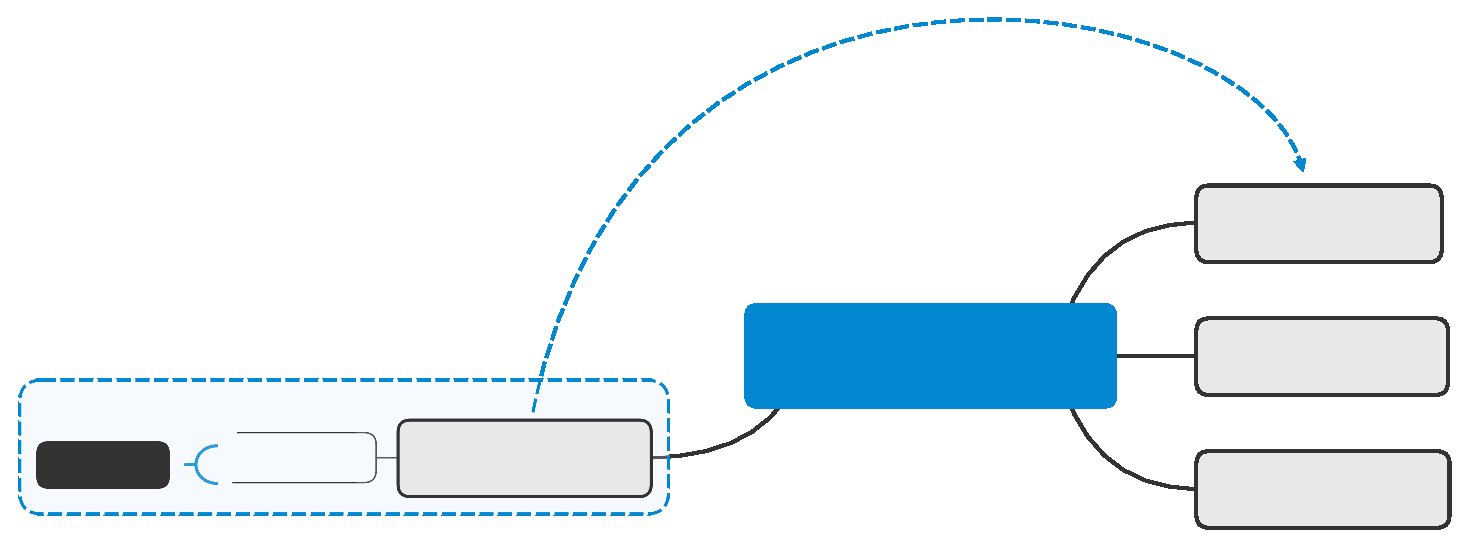
\includegraphics[scale=0.5]{Central_Topic.eps}
    \graphicspath{{/home/ryan/Documents/RYANFAN113/latex_learning/}}
    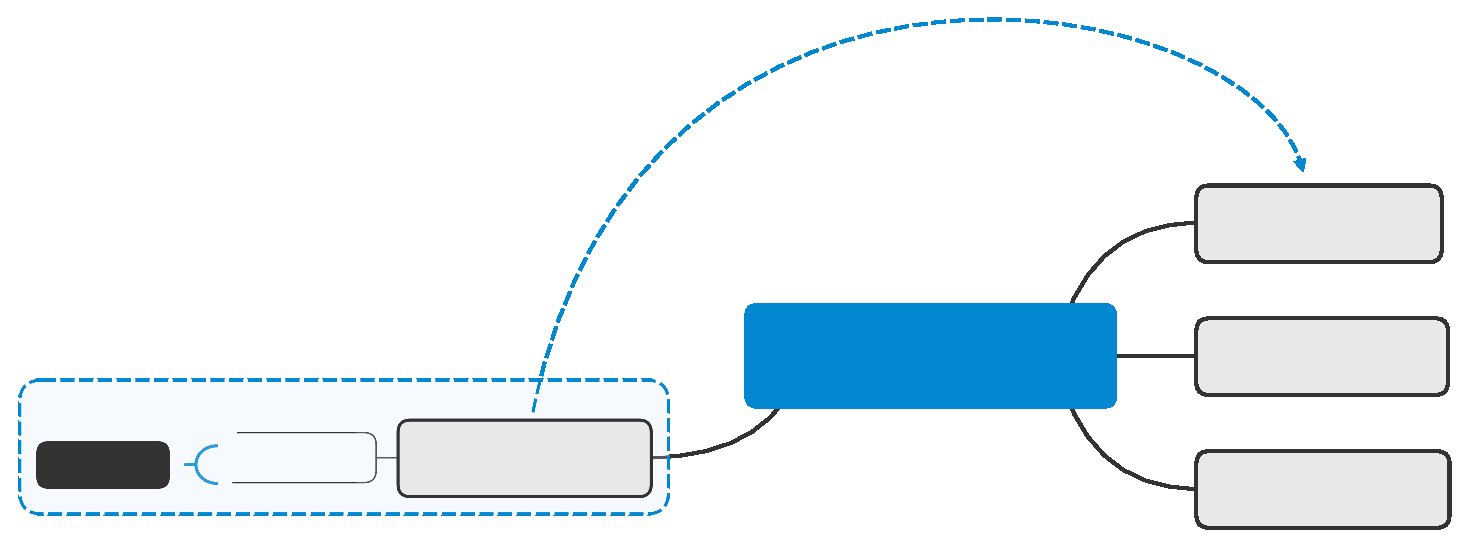
\includegraphics[scale=0.5]{Central_Topic.eps}
    \subsection{盒子}
    \subsubsection{水平盒子}
    \textbackslash mbox\{\ldots \}\par
    \textbackslash makebox$[\langle width\rangle][\langle align\rangle]\{\ldots \}$\par
    \textbackslash mbox 生成一个基本的水平盒子,内容只有一行,不允许分段(除非嵌套其它盒子)
    \textbackslash makebox 更进一步,可以加上可选参数用于控制盒子的宽度 $\langle width\rangle$,%
    以及内容的对齐方式$\langle align\rangle$,可选居中 c(默认值) 、左对齐 l、右对齐 r 和分散对齐 s\par
    |\mbox{Test some words.}|\\
    |\makebox[10em]{Test some words.}|\\
    |\makebox[10em][l]{Test some words.}|\\
    |\makebox[10em][r]{Test some words.}|\\
    |\makebox[10em][s]{Test some words.}|\par
    \subsubsection{带框的水平盒子}
    \textbackslash fbox 和 \textbackslash framebox 让我们可以为水平盒子添加边框。\par
    \fbox{Test some words.}\\
    \framebox[10em][r]{Test some words.}\par
    可以通过 \textbackslash setlength 命令调节边框的宽度 \textbackslash fboxrule %
    和内边距 \textbackslash fboxsep:\par
    \framebox[10em][r]{Test box.}\\
    \setlength{\fboxrule}{1.6pt}
    \setlength{\fboxsep}{1em}
    \framebox[10em][r]{Test box.}\par
    \subsubsection{垂直盒子}
    排版一个文字可以换行的盒子:\par
    \textbackslash parbox$[\langle align\rangle][\langle height\rangle][\langle inner-align\rangle]\{\langle width\rangle\}\{\ldots \}$
    \textbackslash begin\{minipage\}$[\langle align\rangle][\langle height\rangle][\langle inner-align\rangle]\{\langle width\rangle\}$\\
    \ldots\\
    \textbackslash end\{minipage\}\par
    其中 $[\langle align\rangle]$ 为盒子和周围文字的对齐情况(类似 tabular 环境); %
    $\langle height\rangle$ 和 $\langle inner-align\rangle$设置盒子的高度和内容的对齐方式,%
    类似水平盒子 \textbackslash makebox 的设置,不过 $\langle inner-align\rangle$ 接受的%
    参数是顶部 t、底部 b、居中 c 和分散对齐 s。\par
    三字经:\parbox[t]{3em}{人之初 性本善 性相近 习相远}
    \quad
    千字文:
    \begin{minipage}[b][8ex][t]{4em}
        天地玄黄 宇宙洪荒
    \end{minipage}\par
    如果在 minipage 里使用 \textbackslash footnote 命令,生成的脚注会出现在盒子底部,编号是独立的, %
    并且使用小写字母编号。而在 \textbackslash parbox 里无法正常使用 \textbackslash footnote 命令,%
    只能在盒子里使用\textbackslash footnotemark,在盒子外使用\textbackslash footnotetext。\par
    \fbox{这是一个垂直盒子的测试。\footnotemark}
    \footnotetext{注脚来自fbox}
    \fbox{\begin{minipage}{15em}%
             这是一个垂直盒子的测试。
             \footnote{注脚来自minipage.}   
          \end{minipage}
    }\par
    \subsubsection{标尺盒子}
    \textbackslash rule $[\langle raise\rangle]\{\langle width\rangle\}\{\langle height\rangle\}$%
    命令用来画一个实心的矩形盒子,也可适当调整以用来画线(标尺):\par
    Black \rule{12pt}{4pt} box.\\
    Upper \rule[4pt]{6pt}{8pt} and lower \rule[-4pt]{6pt}{8pt} box.\\
    A \rule[-.4pt]{6pt}{.4pt} line.\par
    \subsection{浮动体}
    \LaTeX 预定义了两类浮动体环境 figure 和 table。习惯上 figure 里放图片,table 里放表格,但并没有严格限制,%
    可以在任何一个浮动体里放置文字、公式、表格、图片等等任意内容。\par
    \textbackslash begin\{table\}$[\langle placement\rangle]$\\
    \ldots\\
    \textbackslash end\{table\}\par
    $[\langle placement\rangle]$ 参数提供了一些符号用来表示浮动体允许排版的位置,%
    如 hbp 允许浮动体排版在当前位置、底部或者单独成页。table 和 figure 浮动体的默认设置为 tbp。\par
    双栏排版环境下,\LaTeX 提供了 table* 和 figure* 环境用来排版跨栏的浮动体。它们的用%
    法与 table 和 figure 一样,不同之处为双栏的 $[\langle placement\rangle]$ 参数只能用 tp 两个位置。\par
    \begin{tabular}{ll}
        \toprule
        参数     & 含义\\
        \midrule
        h       & 当前位置(代码所处的上下文)\\
        t       & 顶部\\
        b       & 底部\\ 
        p       & 单独成页\\ 
        !       & 在决定位置时忽视限制\\
        \bottomrule
    \end{tabular}\par
    \textbackslash clearpage 命令 会在另起一页之前,先将所有推迟处理的浮动体排版成页,%
    此时 htbp 等位置限制被完全忽略。\par
    float 宏包为浮动体提供了 H 位置参数,不与 htbp 及 ! 混用。使用 H 位置参数时,%
    会取消浮 动机制,将浮动体视为一般的盒子插入当前位置。\par
    \subsubsection{浮动体的标题}
    图表等浮动体提供了 \textbackslash caption\{\ldots\} 命令加标题,并且自动给浮动体编号:\par
    可以用带星号的命令 \textbackslash caption* 生成不带编号 的标题,%
    也可以使用带可选参数的形式 \textbackslash caption[\ldots]\{\ldots\},
    使得在目录里使用短标题。\textbackslash caption 命令之后还可以紧跟 %
    \textbackslash label 命令标记交叉引用。\par
    可通过修改 \textbackslash figurename 和 \textbackslash tablename %
    的内容来修改标题的前缀。标题样式的 定制功能由 caption 宏包提供.\par
    table 和 figure 两种浮动体分别有各自的生成目录的命令:\\
    \textbackslash listoftables\\
    \textbackslash listoffigures\par    
    \subsubsection{并排和子图表}
    \begin{figure}[htbp]
        \centering
        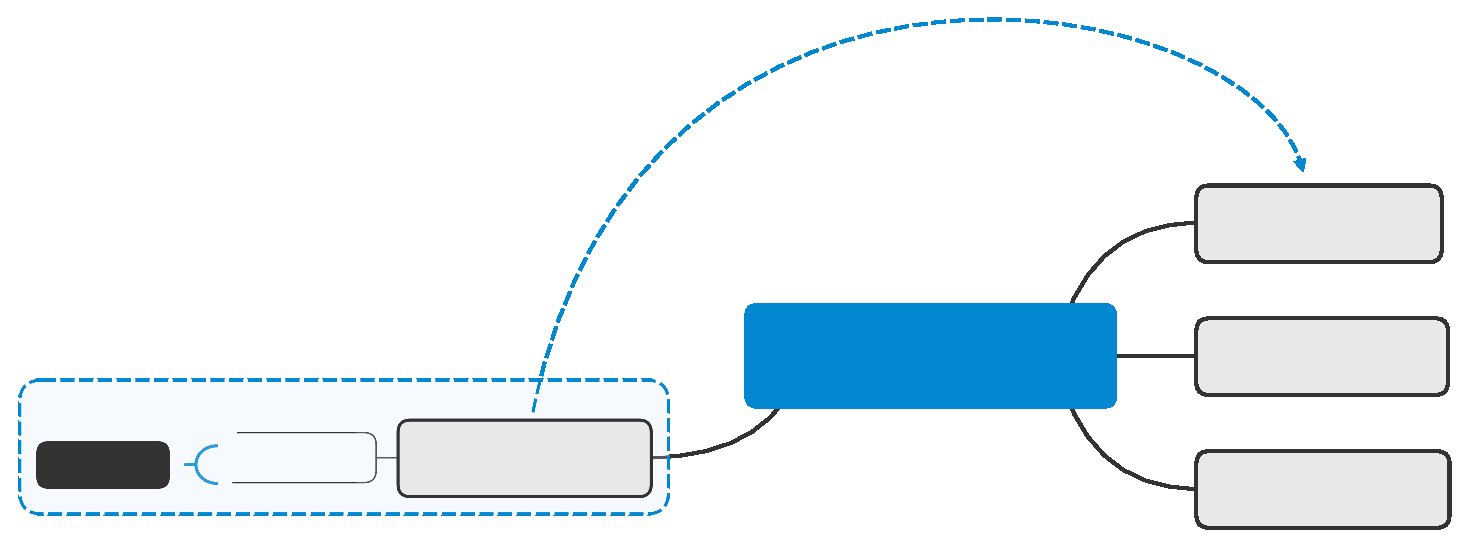
\includegraphics[scale=0.125]{Central_Topic.eps}
        \qquad
        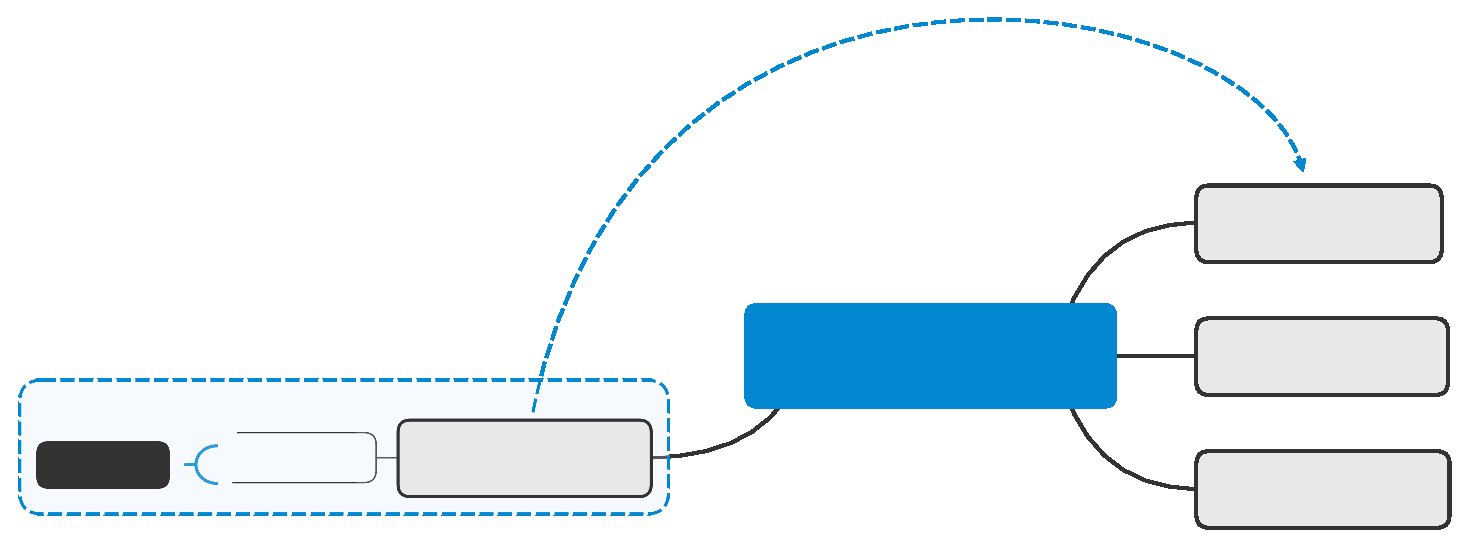
\includegraphics[scale=0.125]{Central_Topic.eps}\\
        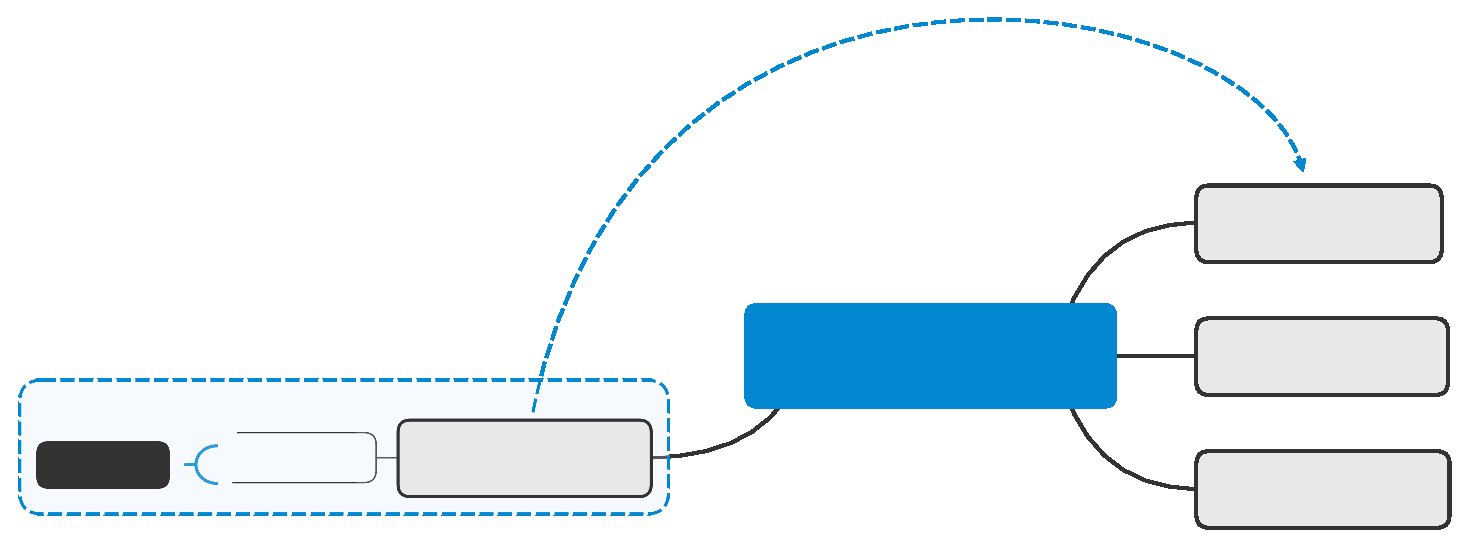
\includegraphics[scale=0.25]{Central_Topic.eps}
        \caption{图片标题}
        \label{}
    \end{figure}
    由于标题是横跨一行的,用 \textbackslash caption 命令为每个图片单独生成标题%
    就需要借助前文提到的\textbackslash parbox 或者 minipage 环境,将标题限制在盒子内。\par
    \begin{figure}[htbp]
        \centering
        \begin{minipage}[b][120pt][t]{0.45\linewidth}
            \centering
            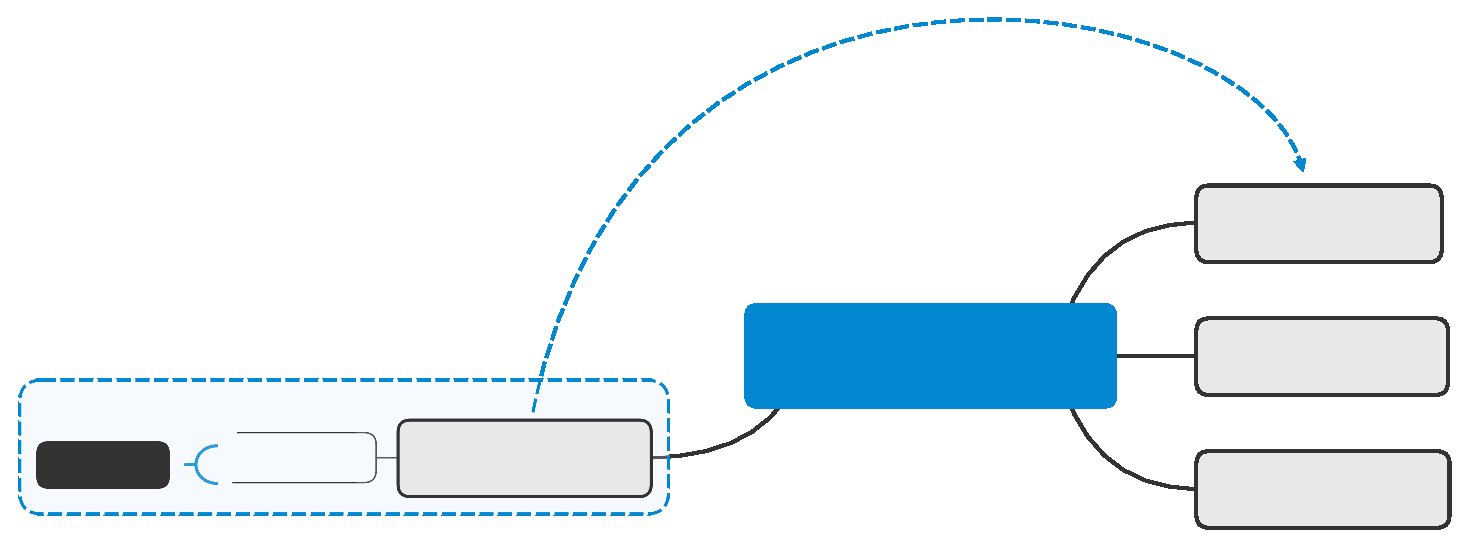
\includegraphics[scale=0.25]{Central_Topic.eps}
            \caption{并排图1}
        \end{minipage}
        \qquad
        \begin{minipage}[b][120pt][t]{0.45\linewidth}
            \centering
            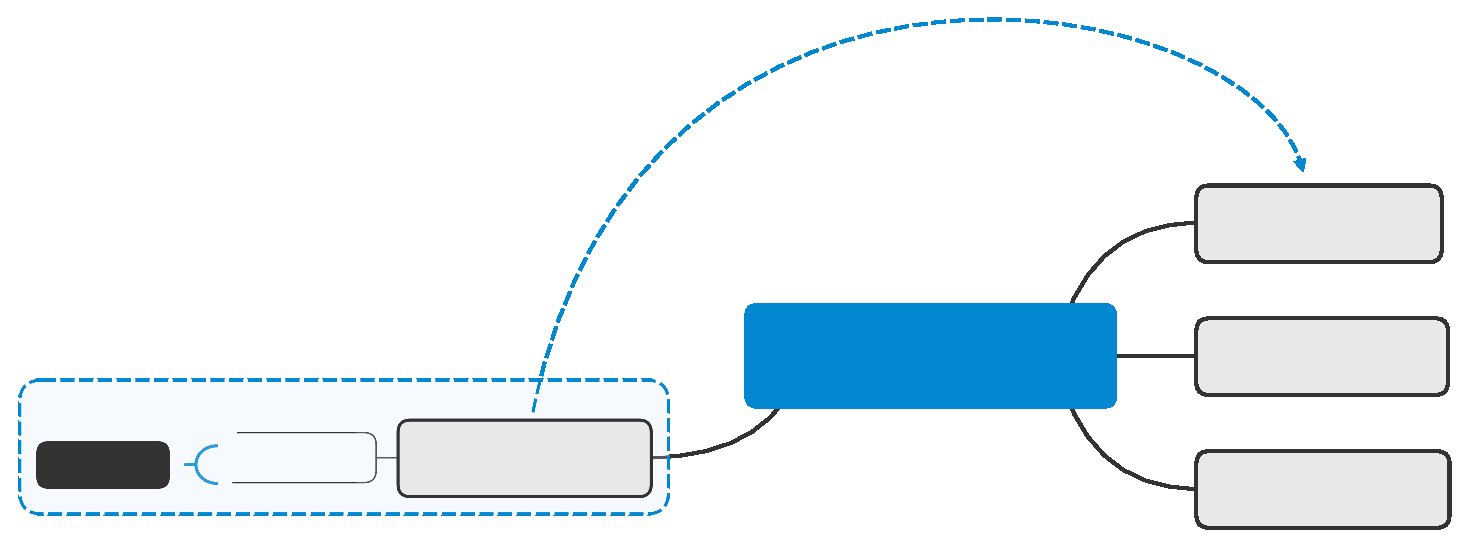
\includegraphics[scale=0.25]{Central_Topic.eps}
            \caption{并排图2}
        \end{minipage}
    \end{figure}     
    给每个图片定义小标题时,就要用到 subfig 宏包的功能    
    \begin{figure}[htbp]
        \centering
        \subfloat[]{%
            \begin{minipage}[b][100pt][t]{0.45\linewidth}
                \centering
                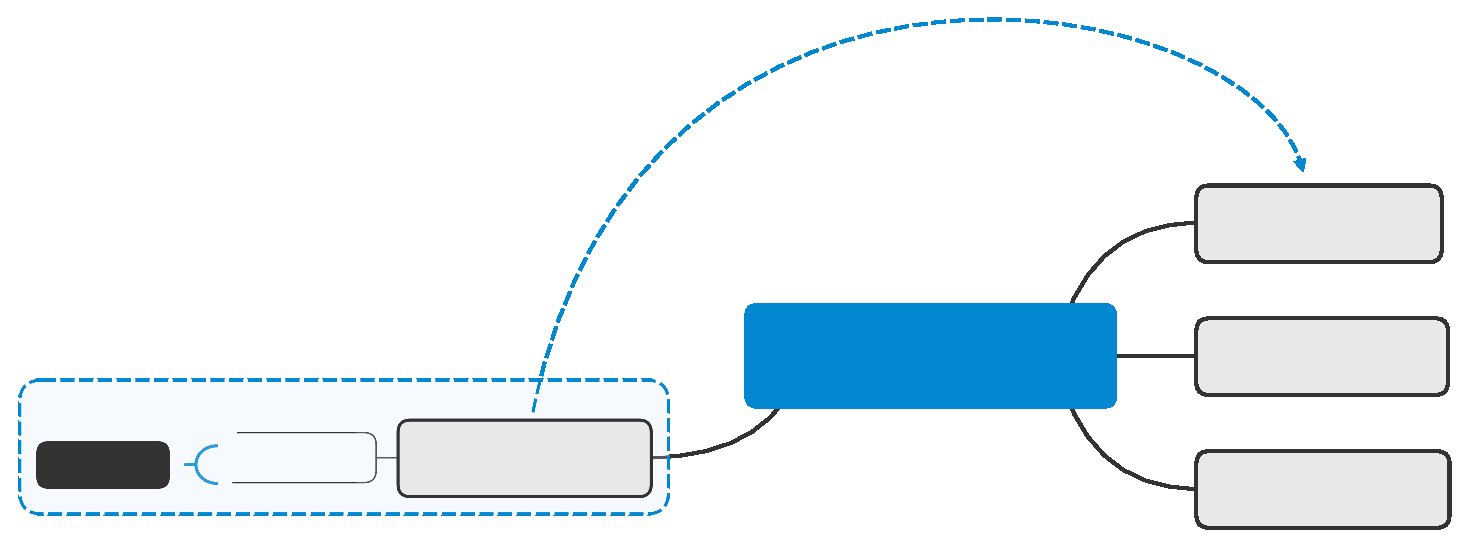
\includegraphics[scale=0.25]{Central_Topic.eps}
            \end{minipage}
        }
        \qquad
        \subfloat[]{%
            \begin{minipage}[b][100pt][t]{0.45\linewidth}
                \centering 
                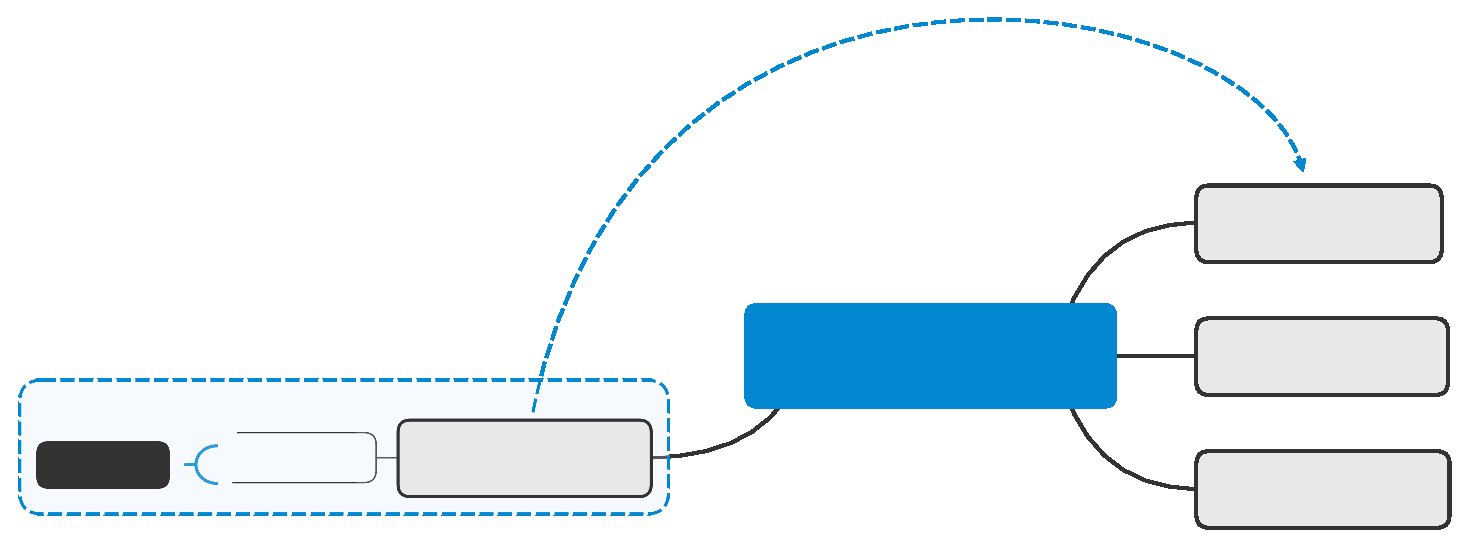
\includegraphics[scale=0.25]{Central_Topic.eps}
            \end{minipage}
        }
        \caption{使用 subfig 宏包的 \textbackslash subfloat 命令排版子图。}
    \end{figure}
    \section{数学公式}
    amsmath 宏 包,对多行公式的排版提供了有力的支持,%
    amsfonts 宏包以及基于它的 amssymb 宏包提 供了丰富的数学符号,%
    amsthm 宏包扩展了 \LaTeX 定理证明格式。\par
    \subsection{公式排版基础}
    \subsubsection{行内和行间公式}
    行内公式由一对 \$ 符号包裹:\\
    The Pythagorean theorem is %
    $a^2 + b^2 = c^2$.\par
    行间公式在 \LaTeX 里由 equation 环境包裹,equation 环境为公式自动生成一 个编号,%
    这个编号可以用 \textbackslash label 和 \textbackslash ref 生成交叉引用。\par
    amsmath 的 \textbackslash eqref 命令甚至为引用 自动加上圆括号;%
    还可以用 \textbackslash tag 命令手动修改公式的编号,%
    或者用 \textbackslash notag 命令取消为公式编 号。\par
    The Pythagorean theorem is:
    \begin{equation}
        a^2 + b^2 = c^2 \label{pythagorean}
    \end{equation}
    Equation \eqref{pythagorean} is called `Gougu theorem' in Chinese.\par
    It's wrong to say
    \begin{equation}
        1 + 1 = 3 \tag{dumb}
    \end{equation}
    or
    \begin{equation}
        1 + 1 = 4 \notag
    \end{equation}\par
    直接使用不带编号的行间公式:
    \begin{equation*}
        a^2 + b^2 = c^2
    \end{equation*}
    For short:
    \[a^2 + b^2 = c^2\]
    Or if you like the long one:
    \begin{displaymath}
        a^2 + b^2 = c^2
    \end{displaymath}
    行内公式和行间公式的对比:\\
    In text:
    $\lim_{n \to \infty} \sum_{k=1}^n \frac{1}{k^2} = \frac{\pi^2}{6}$\\
    In display:
    \[\lim_{n \to \infty} \sum_{k=1}^n \frac{1}{k^2} = \frac{\pi^2}{6}\]
    \subsection{数学模式}
    \renewcommand{\labelenumi}{\arabic{enumi}.}
    \begin{enumerate}
        \item 数学模式中输入的空格被忽略。
        \item 不允许有空行(分段)。
        \item 所有的字母被当作数学公式中的变量处理,想在数学公式中输入正体的文本,%
              可以用\textbackslash mathrm 或者 amsmath 提供的 \textbackslash text 命令。
    \end{enumerate}
    $x^2 \geq 0  \qquad
     \text{for \textbf{all} } x \in \mathbb{R}$
    \subsection{数学符号}
    \subsubsection{一般符号}    
    \begin{table}[H]
        \centering
        \caption{文本/数学模式通用符号}
        \begin{tabular}{clclclcl}
            \hline
            \{      & \textbackslash\{       & \}   & \textbackslash\}    & \$          & \textbackslash\$             & \%     & \textbackslash\%      \\
            \dag    & \textbackslash dag     & \S   & \textbackslash S    & \copyright  & \textbackslash copyright     & \dots  & \textbackslash dots   \\
            \ddag   & \textbackslash ddag    & \P   & \textbackslash P    & \pounds     & \textbackslash pounds        & \S     & \textbackslash S      \\
            \textasteriskcentered   & \textbackslash textasteriskcentered &
            \textperiodcentered     & \textbackslash textperiodcentered   &
            \textbullet             & \textbackslash textbullet           \\
            \textregistered{}       & \textbackslash textregistered{}     &
            \texttrademark          & \textbackslash texttrademark        \\
            \hline
        \end{tabular}        
    \end{table}
    \begin{table}[H]
        \centering
        \caption{希腊字母}
        \begin{tabular}{clclclcl}
            \toprule
            $\alpha$        & \textbackslash alpha      & $\theta$      & \textbackslash theta      &
            $o$             & o                         & $\upsilon$    & \textbackslash upsilon    \\
            $\beta$         & \textbackslash beta       & $\vartheta$   & \textbackslash vartheta   &
            $\pi$           & \textbackslash pi         & $\phi$        & \textbackslash phi        \\
            $\gamma$        & \textbackslash gamma      & $\iota$       & \textbackslash iota       &
            $\varpi$        & \textbackslash varpi      & $\varphi$     & \textbackslash varphi     \\
            $\delta$        & \textbackslash delta      & $\kappa$      & \textbackslash kappa      &
            $\rho$          & \textbackslash rho        & $\chi$        & \textbackslash chi        \\
            $\epsilon$      & \textbackslash epsilon    & $\lambda$     & \textbackslash lambda     &
            $\varrho$       & \textbackslash varrho     & $\psi$        & \textbackslash psi        \\
            $\varepsilon$   & \textbackslash varepsilon & $\mu$         & \textbackslash mu         & 
            $\sigma$        & \textbackslash sigma      & $\omega$      & \textbackslash omega      \\
            $\zeta$         & \textbackslash zeta       & $\nu$         & \textbackslash nu         &
            $\varsigma$     & \textbackslash varsigma                                               \\ 
            $\eta$          & \textbackslash eta        & $\xi$         & \textbackslash xi         & 
            $\tau$          & \textbackslash tau                                                    \\
            \midrule
            $\Gamma$        & \textbackslash Gamma      & $\Lambda$     & \textbackslash Lambda     &
            $\Sigma$        & \textbackslash Sigma      & $\Psi$        & \textbackslash Psi        \\
            $\Delta$        & \textbackslash Delta      & $\Xi$         & \textbackslash Xi         &
            $\Upsilon$      & \textbackslash Upsilon    & $\Omega$      & \textbackslash Omega      \\
            $\Theta$        & \textbackslash Theta      & $\Pi$         & \textbackslash Pi         & 
            $\Phi$          & \textbackslash Phi                                                    \\
            \midrule
            \multicolumn{4}{l}{以下命令依赖 amsmath 宏包}\\
            $\varGamma$     & \textbackslash varGamma   & $\varLambda$  & \textbackslash varLambda  & 
            $\varSigma$     & \textbackslash varSigma   & $\varPsi$     & \textbackslash varPsi     \\
            $\varDelta$     & \textbackslash varDelta   & $\varXi$      & \textbackslash varXi      &
            $\varUpsilon$   & \textbackslash varUpsilon & $\varOmega$   & \textbackslash varOmega   \\
            $\varTheta$     & \textbackslash varTheta   & $\varPi$      & \textbackslash varPi      &
            $\varPhi$       & \textbackslash varPhi                                                 \\
            \midrule
            \multicolumn{4}{l}{依赖 amssymb 宏包}\\
            $\digamma$      & \textbackslash digamma    & $\varkappa$   & \textbackslash varkappa   &
            $\beth$         & \textbackslash beth       & $\gimel$‬      & \textbackslash gimel      \\ 
            $\daleth$       & \textbackslash daleth                                                 \\
            \bottomrule
        \end{tabular}        
    \end{table}
    \begin{table}[H]  
        \centering  
        \caption{其它符号}
        \begin{tabular}{clclclcl}
            \toprule
            $\dots$         & \textbackslash dots       & $\cdots$          & \textbackslash cdots                          &
            $\vdots$        & \textbackslash vdots      & $\ddots$          & \textbackslash ddots                          \\
            $\hbar$         & \textbackslash hbar       & $\imath$          & \textbackslash imath                          &
            $\jmath$        & \textbackslash jmath      & $\ell$            & \textbackslash ell                            \\
            $\Re$           & \textbackslash Re         & $\Im$             & \textbackslash Im                             &
            $\aleph$        & \textbackslash aleph      & $\wp$             & \textbackslash wp                             \\
            $\forall$       & \textbackslash forall     & $\exists$         & \textbackslash exists                         &  
            $\partial$      & \textbackslash partial    & $'$               & '                                             \\ 
            $\prime$        & \textbackslash prime      & $\emptyset$       & \textbackslash emptyset                       &
            $\infty$        & \textbackslash infty      & $\nabla$          & \textbackslash nabla                          \\ 
            $\triangle$     & \textbackslash triangle   & $\bot$            & \textbackslash bot                            &
            $\top$          & \textbackslash top        & $\angle$          & \textbackslash angle                          \\
            $\surd$         & \textbackslash surd       & $\diamondsuit$    & \textbackslash diamondsuit                    &
            $\heartsuit$    & \textbackslash heartsuit  & $\clubsuit$       & \textbackslash clubsuit                       \\ 
            $\spadesuit$    & \textbackslash spadesuit  & $\neg$            & \textbackslash neg or \textbackslash lnot     &
            $\flat$         & \textbackslash flat       & $\natural$        & \textbackslash natural                        \\
            $\sharp$        & \textbackslash sharp                                                                          \\
            \midrule
            \multicolumn{3}{l}{以下命令依赖 latexsym 宏包}\\
            $\mho$          & \textbackslash mho        & $\Box$            & \textbackslash Box                            &
            $\Diamond$      & \textbackslash Diamond                                                                        \\
            \bottomrule
        \end{tabular}    
    \end{table}
    $a_1,a_2,\dots,a_n$\\
    $a_1 + a_2 + \cdots + a_n$\par
    \subsubsection{指数、上下标和导数}
    \textasciicircum 和 \_ 标明上下标。%
    注意上下标的内容(子公式)一般需要用花括号包裹,否 则上下标只对后面的一个符号起作用:\par
    $p^3_{ij} \qquad
     m_\mathrm{Kunth} \qquad
     \sum_{k=1}^3 k$\\
    $a^x +y \neq a^{x+y} \qquad
     e^{x^2} \neq {e^x}^2$ \par
    导数符号$'$ 是一类特殊的上标,可以适当连用表示多阶导数,也可以在其后连用上标:\par
    $f(x) = x^2 \quad
     f'(x) = 2x \quad
     f''^{2}(x) = 4$ \par
    \subsubsection{分式和根式}
    分式使用 \textbackslash frac\{分子\}\{分母\} 来书写。%
    分式的大小在行间公式中是正常大小,而在行内被 极度压缩。%
    amsmath 提供了方便的命令 \textbackslash dfrac 和 \textbackslash tfrac,%
    令用户能够在行内使用正常大小的 分式,或是反过来。\par
    In display style:
    \[
        3/8 \qquad
        \frac{3}{8} \qquad
        \tfrac{3}{8}
    \]
    In text style:
    $1\frac{1}{2}$~hours \qquad
    $1\dfrac{1}{2}$~hours\par
    一般的根式使用 \textbackslash sqrt\{\dots\};%
    表示 n 次方根时写成 \textbackslash sqrt[n]\{\dots\}。\par
    $\sqrt{x} \Leftrightarrow x^{1/2} \quad
     \sqrt[3]{2} \quad
     \sqrt{x^{2} + \sqrt{y}}$ \par
    特殊的分式形式,如二项式结构,由 amsmath 宏包的 \textbackslash binom 命令生成:\par
    Pascal's rule is
    \[
        \binom{n}{k} = \binom{n - 1}{k} + \binom{n - 1}{k}   
    \]
    \subsubsection{关系符}
    \begin{table}[H]
        \centering
        \caption{二元关系符}
        \begin{tabular}{clclcl}
            \toprule
            $<$             & <                         & $>$           & >                                         & 
            $=$             & =                                                                                     \\
            $\equiv$        & \textbackslash equiv      & $\leq$        & \textbackslash leq or \textbackslash le   & 
            $\geq$          & \textbackslash geq or \textbackslash ge                                               \\
            $\ll$           & \textbackslash ll         & $\gg$         & \textbackslash gg                         & 
            $\doteq$        & \textbackslash doteq                                                                  \\
            $\prec$         & \textbackslash prec       & $\succ$       & \textbackslash succ                       &
            $\sim$          & \textbackslash sim                                                                    \\
            $\preceq$       & \textbackslash preceq     & $\succeq$     & \textbackslash succeq                     &
            $\simeq$        & \textbackslash simeq                                                                  \\
            $\subset$       & \textbackslash subset     & $\supset$     & \textbackslash supset                     &
            $\approx$       & \textbackslash approx                                                                 \\
            $\subseteq$     & \textbackslash subseteq   & $\supseteq$   & \textbackslash supseteq                   &
            $\cong$         & \textbackslash cong                                                                   \\
            $\sqsubseteq$   & \textbackslash sqsubseteq & $\sqsupseteq$ & \textbackslash sqsupseteq                 & 
            $\bowtie$       & \textbackslash bowtie                                                                 \\
            $\in$           & \textbackslash in         & $\ni$         & \textbackslash ni ,\textbackslash owns    &
            $\propto$       & \textbackslash propto                                                                 \\
            $\vdash$        & \textbackslash vdash      & $\dashv$      & \textbackslash dashv                      &
            $\models$       & \textbackslash models                                                                 \\
            $\mid$          & \textbackslash mid        & $\parallel$   & \textbackslash parallel                   &
            $\perp$         & \textbackslash perp                                                                   \\
            $\smile$        & \textbackslash smile      & $\frown$      & \textbackslash frown                      &
            $\asymp$        & \textbackslash asymp                                                                  \\
            $:$             & :                         & $\notin$      & \textbackslash notin                      &
            $\neq$          & \textbackslash neq or \textbackslash ne                                               \\
            \midrule
            \multicolumn{3}{l}{以下命令依赖 latexsym 宏包}\\
            $\sqsubset$     & \textbackslash sqsubset   & $\sqsupset$   & \textbackslash sqsupset                   & 
            $\Join$         & \textbackslash Join                                                                   \\
            \midrule 
            \multicolumn{3}{l}{以下命令依赖 amssymb 宏包}\\
            $\lessdot$              & \textbackslash lessdot            & $\gtrdot$         & \textbackslash gtrdot         & 
            $\doteqdot$             & \textbackslash doteqdot                                                               \\
            $\leqslant$             & \textbackslash leqslant           & $\geqslant$       & \textbackslash geqslant       &
            $\risingdotseq$         & \textbackslash risingdotseq                                                           \\
            $\eqslantless$          & \textbackslash eqslantless        & $\eqslantgtr$     & \textbackslash eqslantgtr     &
            $\fallingdotseq$        & \textbackslash fallingdotseq                                                          \\
            $\leqq$                 & \textbackslash leqq               & $\geqq$           & \textbackslash geqq           &
            $\eqcirc$               & \textbackslash eqcirc                                                                 \\
            $\circeq$               & \textbackslash circeq             & $\ggg$            & \textbackslash ggg            &
            $\lll$                  & \textbackslash lll or \textbackslash llless                                           \\
            $\lesssim$              & \textbackslash lesssim            & $\gtrsim$         & \textbackslash gtrsim         &
            $\triangleq$            & \textbackslash triangle                                                               \\
            $\lessapprox$           & \textbackslash lessapprox         & $\gtrapprox$      & \textbackslash gtrapprox      &
            $\bumpeq$               & \textbackslash bumpeq                                                                 \\
            $\lessgtr$              & \textbackslash lessgtr            & $\gtrless$        & \textbackslash gtrless        &
            $\Bumpeq$               & \textbackslash Bumpeq                                                                 \\
            $\lesseqgtr$            & \textbackslash lesseqgtr          & $\gtreqless$      & \textbackslash gtreqless      &
            $\thicksim$             & \textbackslash thicksim                                                               \\
            $\lesseqqgtr$           & \textbackslash lesseqqgtr         & $\gtreqqless$     & \textbackslash gtreqqless     &
            $\thickapprox$          & \textbackslash thickapprox                                                            \\
            $\preccurlyeq$          & \textbackslash preccurlyeq        & $\succcurlyeq$    & \textbackslash succcurlyeq    &
            $\approxeq$             & \textbackslash approxeq                                                               \\
            $\curlyeqprec$          & \textbackslash curlyeqprec        & $\curlyeqsucc$    & \textbackslash curlyeqsucc    &
            $\backsim$              & \textbackslash backsim                                                                \\
            $\precsim$              & \textbackslash precsim            & $\succsim$        & \textbackslash succsim        &
            $\backsimeq$            & \textbackslash backsimeq                                                              \\
            $\precapprox$           & \textbackslash precapprox         & $\succapprox$     & \textbackslash succapprox     &
            $\vDash$                & \textbackslash vDash                                                                  \\
            $\subseteqq$            & \textbackslash subseteqq          & $\supseteqq$      & \textbackslash supseteqq      &
            $\Vdash$                & \textbackslash Vdash                                                                  \\
            $\shortparallel$        & \textbackslash shortparallel      & $\Supset$         & \textbackslash Supset         &
            $\Vvdash$               & \textbackslash Vvdash                                                                 \\
            $\blacktriangleleft$    & \textbackslash blacktriangleleft  & $\sqsupset$       & \textbackslash sqsupset       &
            $\backepsilon$          & \textbackslash backepsilon                                                            \\
            $\vartriangleright$     & \textbackslash vartriangleright   & $\because$        & \textbackslash because        &
            $\varpropto$            & \textbackslash varpropto                                                              \\
            $\blacktriangleright$   & \textbackslash blacktriangleright & $\Subset$         & \textbackslash Subset         &
            $\between$              & \textbackslash between                                                                \\
            $\trianglerighteq$      & \textbackslash trianglerighteq    & $\smallfrown$     & \textbackslash smallfrown     &
            $\pitchfork$            & \textbackslash pitchfork                                                              \\
            $\vartriangleleft$      & \textbackslash vartriangleleft    & $\shortmid$       & \textbackslash shortmid       &
            $\smallsmile$           & \textbackslash smallsmile                                                             \\
            $\trianglelefteq$       & \textbackslash trianglelefteq     & $\therefore$      & \textbackslash therefore      &
            $\sqsubset$             & \textbackslash sqsubset                                                               \\
            \bottomrule
        \end{tabular}
    \end{table}
    \LaTeX 还提供了自定义二元关系符的命令 \textbackslash stackrel,用于将一个符号叠加在原有的二元关 系符之上:\par
    \[
        f_n(x) \stackrel{*}{\approx} 1    
    \]
    \subsubsection{算符}
    \begin{table}[H]
        \centering
        \caption{二元运算符}
        \begin{tabular}{clclcl}
            \toprule
            $+$                 & +                         &$-$                    & -                                 &         
            $\pm$               & \textbackslash pm                                                                     \\
            $\mp$               & \textbackslash mp         & $\triangleleft$       & \textbackslash triangleleft       &
            $\cdot$             & \textbackslash cdot                                                                   \\
            $\div$              & \textbackslash div        & $\triangleright$      & \textbackslash triangleright      &
            $\times$            & \textbackslash times                                                                  \\
            $\setminus$         & \textbackslash setminus   & $\star$               & \textbackslash star               &
            $\cup$              & \textbackslash cup                                                                    \\
            $\cap$              & \textbackslash cap        & $\ast$                & \textbackslash ast                &
            $\sqcup$            & \textbackslash sqcup                                                                  \\
            $\sqcap$            & \textbackslash sqcap      & $\circ$               & \textbackslash circ               &
            $\vee$              & \textbackslash vee                                                                    \\
            $\lor$              & \textbackslash lor        & $\wedge$              & \textbackslash wedge              &
            $\land$             & \textbackslash land                                                                   \\
            $\bullet$           & \textbackslash bullet     & $\oplus$              & \textbackslash oplus              &
            $\ominus$           & \textbackslash ominus                                                                 \\
            $\diamond$          & \textbackslash diamond    & $\odot$               & \textbackslash odot               &
            $\oslash$           & \textbackslash oslash                                                                 \\
            $\uplus$            & \textbackslash uplus      & $\otimes$             & \textbackslash otimes             &
            $\bigcirc$          & \textbackslash bigcirc                                                                \\
            $\amalg$            & \textbackslash amalg      & $\bigtriangleup$      & \textbackslash bigtriangleup      &
            $\bigtriangledown$  & \textbackslash bigtriangledown                                                        \\
            $\dagger$           & \textbackslash dagger     & $\ddagger$            & \textbackslash ddagger            &
            $\wr$               & \textbackslash wr                                                                     \\
            \midrule
            \multicolumn{3}{l}{以下命令依赖 latexsym 宏包} \\
            $\lhd$              & \textbackslash lhd        & $\rhd$                & \textbackslash rhd                \\
            $\unlhd$            & \textbackslash unlhd      & $\unrhd$              & \textbackslash unrhd              \\
            \midrule
            \multicolumn{3}{l}{以下命令依赖 amssymb 宏包} \\
            $\dotplus$          & \textbackslash dotplus        & $\centerdot$      & \textbackslash centerdot          \\
            $\ltimes$           & \textbackslash ltimes         & $\rtimes$         & \textbackslash rtimes             &
            $\divideontimes$    & \textbackslash divideontimes                                                          \\
            $\doublecup$        & \textbackslash doublecup      & $\doublecap$      & \textbackslash doublecap          &
            $\smallsetminus$    & \textbackslash smallsetminus                                                          \\
            $\veebar$           & \textbackslash veebar         & $\barwedge$       & \textbackslash barwedge           &
            $\doublebarwedge$   & \textbackslash doublebarwedge                                                         \\
            $\boxplus$          & \textbackslash boxplus        & $\boxminus$       & \textbackslash boxminus           &
            $\circleddash$      & \textbackslash circleddash                                                            \\
            $\boxtimes$         & \textbackslash boxtimes       & $\boxdot$         & \textbackslash boxdot             &
            $\circledcirc$      & \textbackslash circledcirc                                                            \\
            $\intercal$         & \textbackslash intercal       & $\circledast$     & \textbackslash circledast         &
            $\rightthreetimes$  & \textbackslash rightthreetimes                                                        \\
            $\curlyvee$         & \textbackslash curlyvee       & $\curlywedge$     & \textbackslash curlywedge         &
            $\leftthreetimes$   & \textbackslash listoffigures                                                          \\
            \bottomrule
        \end{tabular}
    \end{table}
    \begin{table}[H]
        \centering
        \caption{\LaTeX 作为算符的函数名称}
        \begin{tabular}{clclclcl}
            \toprule
            \multicolumn{8}{l}{不带上下限的算符}\\
            $\sin$          & \textbackslash sin        & $\arcsin$         & \textbackslash arcsin         &
            $\sinh$         & \textbackslash sinh       & $\exp$            & \textbackslash exp            \\
            $\dim$          & \textbackslash dim        & $\cos$            & \textbackslash cos            & 
            $\arccos$       & \textbackslash arccos     &$\cosh$            & \textbackslash cosh           \\
            $\log$          & \textbackslash log        & $\ker$            & \textbackslash ker            & 
            $\tan$          & \textbackslash tan        & $\arctan$         & \textbackslash arctan         \\
            $\tanh$         & \textbackslash tanh       & $\lg$             & \textbackslash lg             &
            $\hom$          & \textbackslash hom        & $\cot$            & \textbackslash cot            \\
            $\arg$          & \textbackslash arg        & $\coth$           & \textbackslash coth           &
            $\ln$           & \textbackslash ln         & $\deg$            & \textbackslash deg            \\
            $\sec$          & \textbackslash sec        & $\csc$            & \textbackslash csc            \\
            \midrule
            \multicolumn{8}{l}{带上下限的算符}\\
            $\lim$          & \textbackslash lim        & $\limsup$         & \textbackslash limsup         &
            $\liminf$       & \textbackslash liminf     & $\sup$            & \textbackslash sup            \\
            $\inf$          & \textbackslash inf        & $\min$            & \textbackslash min            &
            $\max$          & \textbackslash max        & $\det$            & \textbackslash det            \\
            $\Pr$           & \textbackslash Pr         & $\gcd$            & \textbackslash gcd            \\         
            \bottomrule
        \end{tabular}
    \end{table}
    \[
        \lim_{x \rightarrow 0} \frac{\sin x}{s} = 1    
    \]
    对于求模表达式,\LaTeX 提供了 \textbackslash pmod 和 \textbackslash bmod 命令:\par
    \[
        a \bmod b   \qquad
        x \equiv a \pmod{b}  
    \]
    amsmath 允许用户在\emph{导言区}用 \textbackslash DeclareMathOperator 在定义自己 的算符,%
    其中带星号的命令定义带上下限的算符:\\
    \[ \argh 3 = \nut_{x = 1} 4x \]
    \subsubsection{巨算符}
    In text:
    $
        \sum_{i=1}^n   \quad
        \int_0^{\frac{\pi}{2}}   \quad
        \oint_0^{\frac{\pi}{2}} \quad
        \prod_{\epsilon}
    $\\
    In display:
    \[
        \sum_{i=1}^n    \quad 
        \int_0^{\frac{\pi}{2}}\quad
        \oint_0^{\frac{\pi}{2}} \quad 
        \prod_{\epsilon}    
    \]\par
    巨算符的上下标位置可由 \textbackslash limits 和 \textbackslash nolimits 控制\par
    In text:
    $
        \sum\limits_{i=1}^n \quad
        \int\limits_0^{\frac{\pi}{2}}   \quad
        \oint\limits_0^{\frac{\pi}{2}}  \quad
        \prod\limits_{\epsilon}
    $\\
    In display:
    \[
        \sum\nolimits_{i = 1}^n \quad
        \int\limits_0^{\frac{\pi}{2}} \quad
        \oint\limits_0^{\frac{\pi}{2}} \quad
        \prod\nolimits_{\epsilon}    
    \]\par
    amsmath 宏包还提供了 \textbackslash substack,能够在下限位置书写多行表达式:
    \[
        \sum_{\substack{0\le i\le n\\
                        j\in\mathbb{R}}} P(i,j) = Q(n)    
    \]
    subarray 环境更进 一步,令多行表达式可选择居中 (c) 或左对齐 (l):
    \[
        \sum_{\begin{subarray}{l}
                    0\le i\le n\\
                    j\in\mathbb{R}
              \end{subarray}} P(i,j) = 
        Q(n)
    \]
    \subsubsection{数学重音和上下括号}
    \begin{table}[H]
        \centering
        \caption{数学重音符号}
        \begin{tabular}{clclcl}
            \toprule
            $\hat{a}$           & \textbackslash hat\{a\}           & $\check{a}$           & \textbackslash check\{a\}             &
            $\tilde{a}$         & \textbackslash tilde\{a\}                                                                         \\
            $\acute{a}$         & \textbackslash acute\{a\}         & $\grave{a}$           & \textbackslash grave\{a\}             &
            $\breve{a}$         & \textbackslash breve\{a\}                                                                         \\
            $\bar{a}$           & \textbackslash bar\{a\}           & $\vec{a}$             & \textbackslash vec\{a\}               &
            $\mathring{a}$      & \textbackslash mathring\{a\}                                                                      \\
            $\dot{a}$           & \textbackslash dot\{a\}           & $\ddot{a}$            & \textbackslash ddot\{a\}              \\
            $\widehat{AAA}$     & \textbackslash widehat\{AAA\}     & $\widetilde{AAA}$     & \textbackslash widetilde\{AAA\}       \\
            \midrule
            \multicolumn{6}{l}{以下命令依赖 amsmath 宏包}\\
            $\dddot{a}$         & \textbackslash dddot\{a\}         & $\ddddot{a}$          & \textbackslash ddddot\{a\}            \\
            \midrule
            \multicolumn{6}{l}{以下命令依赖 yhmath 宏包}\\
            $\wideparen{AAA}$   & \textbackslash wideparen\{AAA\}                                                                   \\    
            \bottomrule
        \end{tabular}
    \end{table}
    使用时要注意 重音符号的作用区域,一般应当对某个符号而不是``符号加下标''使用重音:
    \[\bar{x_0} \quad \bar{x}_0 \]
    \[\vec{x_0} \quad \vec{x}_0 \]
    \[\hat{\mathbf{e}_x} \quad \hat{\mathbf{e}}_x \]
    \LaTeX 也能为多个字符加重音,包括直接画线的 \textbackslash overline 和 %
    \textbackslash underline 命令(可叠加使 用)、宽重音符号 \textbackslash widehat、%
    表示向量的箭头 \textbackslash overrightarrow 等。\par
    \begin{table}[H]
        \centering
        \caption{作为重音的箭头符号}
        \begin{tabular}{clcl}
            \toprule
            $\overrightarrow{AB}$           & \textbackslash overrightarrow\{AB\}           &
            $\overleftarrow{AB}$            & \textbackslash overleftarrow\{AB\}            \\
            \midrule
            \multicolumn{4}{l}{以下命令依赖 amsmath 宏包}\\
            $\underleftarrow{AB}$           & \textbackslash underleftarrow\{AB\}           &
            $\underrightarrow{AB}$          & \textbackslash underrightarrow\{AB\}          \\
            $\overleftrightarrow{AB}$       & \textbackslash overleftrightarrow\{AB\}       &
            $\underleftrightarrow{AB}$      & \textbackslash underleftrightarrow\{AB\}      \\
            \bottomrule
        \end{tabular}
    \end{table}
    \[0.\overline{3} = \underline{\underline{1/3}} \]
    \[\hat{XY} \qquad \widehat{XY} \]
    \[\vec{AB} \qquad \overrightarrow{AB} \]
    \textbackslash overbrace 和 \textbackslash underbrace 命令用来生成上/下括号,各自可带一个上/下标公式:
    \[
        \underbrace{\overbrace{a + b + c}^6 \cdot 
                    \overbrace{d + e + f}^7
                    }_\text{meaning of life} = 
        42
    \]
    \subsubsection{箭头}
    \begin{table}[H]
        \centering
        \caption{箭头}
        \begin{tabular}{clcl}
            $\leftarrow$            & \textbackslash leftarrow or  \textbackslash gets  & $\longleftarrow$            & \textbackslash longleftarrow        \\
            $\rightarrow$           & \textbackslash rightarrow or \textbackslash to    & $\longrightarrow$           & \textbackslash longrightarrow       \\
            $\leftrightarrow$       & \textbackslash leftrightarrow                     & $\longleftrightarrow$       & \textbackslash longleftrightarrow   \\
            $\Leftarrow$            & \textbackslash Leftarrow                          & $\Longleftarrow$            & \textbackslash Longleftarrow        \\
            $\Rightarrow$           & \textbackslash Rightarrow                         & $\Longrightarrow$           & \textbackslash Longrightarrow       \\
            $\Leftrightarrow$       & \textbackslash Leftrightarrow                     & $\Longleftrightarrow$       & \textbackslash Longleftrightarrow   \\
            $\mapsto$               & \textbackslash mapsto                             & $\longmapsto$               & \textbackslash longmapsto           \\
            $\hookleftarrow$        & \textbackslash hookleftarrow                      & $\hookrightarrow$           & \textbackslash hookrightarrow       \\
            $\leftharpoonup$        & \textbackslash leftharpoonup                      & $\rightharpoonup$           & \textbackslash rightharpoonup       \\
            $\leftharpoondown$      & \textbackslash leftharpoondown                    & $\rightharpoondown$         & \textbackslash rightharpoondown     \\
            $\rightleftharpoons$    & \textbackslash rightleftharpoons                  & $\iff$                      & \textbackslash iff                  \\
            $\uparrow$              & \textbackslash uparrow                            & $\downarrow$                & \textbackslash downarrow            \\
            $\updownarrow$          & \textbackslash updownarrow                        & $\Uparrow$                  & \textbackslash Uparrow              \\
            $\Downarrow$            & \textbackslash Downarrow                          & $\Updownarrow$              & \textbackslash Updownarrow          \\
            $\nearrow$              & \textbackslash nearrow                            & $\searrow$                  & \textbackslash searrow              \\
            $\swarrow$              & \textbackslash swarrow                            & $\nwarrow$                  & \textbackslash nwarrow              \\
            \midrule
            \multicolumn{4}{l}{以下命令依赖 latexsym 宏包} \\
            $\leadsto$              & \textbackslash leadsto                                                                                                \\
            \bottomrule
        \end{tabular}
    \end{table}
    amsmath 的 \textbackslash xleftarrow 和 \textbackslash xrightarrow 命令%
    提供了长度可以伸展的箭头,并且可以为 箭头增加上下标:
    \[ a\xleftarrow{x + y + z} b \]
    \[ c\xrightarrow[x < y]{a*b*c} d \]
    \subsubsection{括号和定界符}
    \begin{table}[H]
        \centering
        \caption{定界符}
        \begin{tabular}{clclcl}
            \toprule
            $($                 & (                               & $)$                 & )                                 &
            $\uparrow$          & \textbackslash uparrow                                                                    \\
            $[$                 & \textbackslash lbrack or [      & $]$                 & \textbackslash rbrack or ]        &
            $\downarrow$        & \textbackslash downarrow                                                                  \\
            $\{$                & \textbackslash lbrace or \textbackslash\{                                                 & 
            $\}$                & \textbackslash rbrace or \textbackslash\}                                                 &
            $\updownarrow$      & \textbackslash updownarrow                                                                \\
            $\langle$           & \textbackslash langle           & $\rangle$           & \textbackslash rangle             &
            $\Uparrow$          & \textbackslash Uparrow                                                                    \\
            $\vert$             & \textbackslash or |             & $\Downarrow$        & \textbackslash Downarrow          &
            $\|$                & \textbackslash Vert or \textbackslash|                                                    \\
            $/$                 & /                               & $\backslash$        & \textbackslash backslash          &
            $\Updownarrow$      & \textbackslash Updownarrow                                                                \\
            $\lfloor$           & \textbackslash lfloor           & $\rfloor$           & \textbackslash rfloor             &
            $\rceil$            & \textbackslash rceil                                                                      \\
            $\lceil$            & \textbackslash lceil                                                                      \\
            \bottomrule
        \end{tabular}
    \end{table}
    \begin{table}[H]
        \centering
        \caption{用于行间公式的大定界符}
        \begin{tabular}{clcl}
            \toprule
            $\left\lgroup\right.$           & \textbackslash lgroup         & 
            $\left\arrowvert\right.$        & \textbackslash arrowvert      \\
            $\left\rgroup\right.$           & \textbackslash rgroup         &
            $\left\Arrowvert\right.$        & \textbackslash Arrowvert      \\ 
            $\left\lmoustache\right.$       & \textbackslash lmoustache     &
            $\left\bracevert\right.$        & \textbackslash bracevert      \\
            $\left\rmoustache\right.$       & \textbackslash rmoustache     \\
            \bottomrule
        \end{tabular}
    \end{table}
    \[ {a,b,c} \neq \{a,b,c\} \]
    使用 \textbackslash left 和 \textbackslash right 命令可令括号(定界符)的大小可变,在行间公式中常用。%
    \LaTeX 会自动根据括号内的公式大小决定定界符大小。\\
    \textbackslash left 和 \textbackslash right 必须成对使用。需要使用单个定 界符时,另一个定界符写成%
    \textbackslash left. 或 \textbackslash right.\par
    \[
        1 + \left( \frac{1}{1 - x^2} \right)^3  \qquad
        \left.\frac{\partial f}{\partial t} \right|_{t = 0} 
    \]
    还可以用 \textbackslash big、\textbackslash bigg 等命令生成固定大小的定界符。\\
    更常用的形式是类似 \textbackslash left 的 \textbackslash bigl、\textbackslash biggl 等,%
    以及类似 \textbackslash right 的 \textbackslash bigr、\textbackslash biggr 等%
    (\textbackslash bigl 和 \textbackslash bigr 不必成对出现)。\par
    \[ \Bigl((x + 1)(x - 1)\Bigr)^2 \]
    \[  \bigl( \Bigl( \biggl( \Biggl( \quad 
        \bigr\} \Bigr\} \biggr\} \Biggr\} \quad
        \big\| \Big\| \bigg\| \Bigg\| \quad
        \big\Downarrow \Big\Downarrow
        \bigg\Downarrow \Bigg\Downarrow
    \]
    \subsection{多行公式}
    \subsubsection{长公式折行}
    amsmath 宏包的 multline 环境提供了书写折行长公式的方便环境。它允许用 %
    \textbackslash\textbackslash 折行,将 公式编号放在最后一行。%
    多行公式的首行左对齐,末行右对齐,其余行居中。
    \begin{multline}
        a + b + c + d + e + f + g + h + i\\
        = j + k + l + m + n\\
        = o + p + q + r + s\\
        = t + u + v + w + x
    \end{multline}
    类似 equation*,multline* 环境排版不带编号的折行长公式。
    \subsubsection{多行公式}
    罗列一系列公式,并令其按照等号对齐。\\
    目前最常用的是 align 环境,它将公式用 \& 隔为两部分并对齐。分隔符通常放在等号左边:
    \begin{align}
        a & = b + c \\
          & = d + c
    \end{align}
    align 环境会给每行公式都编号。我们仍然可以用 \textbackslash notag 去掉某行的编号。\\
    为了对齐加号,我们将分隔符放在等号右边,这时需要给等号后添加一对括号 \{\} 以产生正常的 间距:
    \begin{align}
        a ={} & b + c   \\
          ={} & d + e + f + g + h + i + j + k + l \notag    \\
              & + m + n + o \\
          ={} & p + q + r + s   
    \end{align}
    align 还能够对齐多组公式,除等号前的 \& 之外,公式之间也用 \& 分隔:
    \begin{align}
        a & = 1     & b & = 2   & c & = 3   \\
        d & = - 1   & e & = - 2 & f & = - 5 
    \end{align}
    如果我们不需要按等号对齐,只需罗列数个公式, gather 将是一个很好用的环境:
    \begin{gather}
        a = b + c   \\
        d = e + f + g   \\
        h + i = j + k   \\
        l + m = n
    \end{gather}
    align 和 gather 有对应的不带编号的版本 align* 和 gather*
    \subsubsection{公用编号的多行公式}
    多个公式组在一起公用一个编号,编号位于公式的居中位置。\\
    amsmath 宏包提供了诸如 aligned、gathered 等环境,%
    与 equation 环境套用。以 -ed 结尾的环境用法与前一节不以 -ed 结尾的环境用法一一对应。
    \begin{equation}
        \begin{aligned}
            a & = b + c \\
            d & = e + f + g   \\
            h + i & = j + k   \\
            l + m & = n
        \end{aligned}
    \end{equation}
    split 环境和 aligned 环境用法类似,也用于和 equation 环境套用,区别是 split 只能 将每行的一个公式分两栏,
    aligned 允许每行多个公式多栏。
    \subsection{数组和矩阵}
    二维数组,\LaTeX 提供了 array 环境,用法与 tabular 环境极为类似,%
    也需要定 义列格式,并用 \textbackslash \textbackslash 换行。%
    数组可作为一个公式块,在外套用 \textbackslash left、\textbackslash right 等定界符:
    \[
        \mathbf{X} = \left(
            \begin{array}{cccc}
                x_{11} & x_{12} & \ldots & x_{1n}   \\
                x_{21} & x_{22} & \ldots & x_{2n}   \\
                \vdots & \vdots & \ddots & \vdots   \\
                x_{n1} & x_{n2} & \ldots & x_{nn}
            \end{array}    
        \right)  
    \]
    amsmath 提供的 cases 环境
    \[
        |x| =
        \begin{cases}
            - x & \text{if } x < 0, \\
            0   & \text{if } x = 0, \\
            x   & \text{if } x > 0.
        \end{cases}
    \]
    amsmath 宏包提供了多种排版矩阵的环境,包括不带定界符的 matrix,以及带各种定界符的矩阵 pmatrix ($\left(\right.$) 、
    bmatrix ($\left[\right.$) 、 Bmatrix ($\left\{\right.$) 。使用这些环境时,无需给定列格式 :
    \[
        \begin{matrix}
            1 & 2   \\
            3 & 4
        \end{matrix}    \qquad
        \begin{bmatrix}
            x_{11} & x_{12} & \ldots & x_{1n} \\
            x_{21} & x_{22} & \ldots & x_{2n} \\
            \vdots & \vdots & \ddots & \vdots \\
            x_{n1} & x_{n2} & \ldots & x_{nn}
        \end{bmatrix}
    \]
    在矩阵中的元素里排版分式时,一来要用到 \textbackslash dfrac 等命令,%
    二来行与行之间有可能紧贴着, 这时要调节间距:
    \[
        \mathbf{H} =
        \begin{bmatrix}
            \dfrac{\partial^2 f}{\partial x^2}         & \dfrac{\partial^2 f}{\partial x\partial y} \\[8pt]
            \dfrac{\partial^2 f}{\partial x\partial y} & \dfrac{\partial^2 f}{\partial y^2}
        \end{bmatrix}    
    \]
    \subsection{公式中的间距}
    生成间距的命令 \textbackslash quad 和 \textbackslash qquad 和 \textbackslash , 在文本和数学 环境中可用\\
    \textbackslash ,、\textbackslash :、\textbackslash ; 以及负间距 \textbackslash ! %
    命令只用于数学环境。文本中的 \textbackslash\verb*| | 也能使用在数学公式中。\par
    \begin{table}[H]
        \centering
        \begin{tabular}{ll|ll}
            \hline
            无额外间距                    &   aa          &   
            \textbackslash ,            &   a\,a        \\
            \textbackslash quad         &   a\quad a    &
            \textbackslash :            &   a\:a        \\
            \textbackslash qquad        &   a\qquad a   &
            \textbackslash ;            &   a\;a        \\
            \textbackslash \verb*| |    &   a\ a        &
            \textbackslash !            &   a\!a        \\
            \hline
        \end{tabular}
    \end{table}
    一个常见的用途是修正积分的被积函数 $f(x)$ 和微元 $\text{d}x$ 之间的距离。
    \[
        \int_a^b f(x) \mathrm{d}x
        \qquad
        \int_a^b f(x) \, \mathrm{d}x    
    \]
    另一个用途是生成多重积分号。如果我们直接连写两个 \textbackslash int,%
    之间的间距将会过宽,此时 可以使用负间距 \textbackslash ! 修正之。    
    \begin{gather*}
        \int\int f(x)g(y) \,\mathrm{d}x\,\mathrm{d}y    \\
        \int\!\!\!\int f(x)g(y) \mathrm{d}\,x\mathrm{d}\,y
    \end{gather*}
    amsmath 提供了更方便的多重积分号,如二重积分 \textbackslash iint、%
    三 重积分 \textbackslash iiint 等。
    \begin{gather*}
        \iint f(x)g(y) \,\mathrm{d}x\,\mathrm{d}y   \\
        \iint \quad \iiint \quad \idotsint
    \end{gather*}
    \subsection{数学符号的字体控制}
    \subsubsection{数学字母字体}
    \begin{table}[H]
        \centering
        \caption{数学字母字体}
        \begin{tabular}{lll}
            \toprule
            示例 &命令 &依赖的宏包\\
            \midrule
            $\mathnormal{ABCDEabcde1234}$   & \textbackslash mathnormal\{\ldots\}   &                     \\
            $\mathrm{ABCDEabcde1234}$       & \textbackslash mathrm\{\ldots\}       &                     \\
            $\mathit{ABCDEabcde1234}$       & \textbackslash mathit\{\ldots\}       &                     \\
            $\mathbf{ABCDEabcde1234}$       & \textbackslash mathbf\{\ldots\}       &                     \\
            $\mathsf{ABCDEabcde1234}$       & \textbackslash mathsf\{\ldots\}       &                     \\
            $\mathtt{ABCDEabcde1234}$       & \textbackslash mathtt\{\ldots\}       &                     \\
            $\mathcal{ABCDEabcde1234}$      & \textbackslash mathcal\{\ldots\}      & 只大写字母            \\
            \midrule
            $\mathcal{ABCDE}$               & \textbackslash mathcal\{\ldots\}      & eucal,只大写字母      \\
            $\mathscr{ABCDE}$               & \textbackslash mathscr\{\ldots\}      & mathrsfs,只大写字母   \\
            $\mathfrak{ABCDEabcde1234}$     & \textbackslash mathfrak\{\ldots\}     & amssymb 或 eufrak    \\
            $\mathbb{ABCDE}$                & \textbackslash mathbb\{\ldots\}       & amssymb,只大写字母    \\
            \bottomrule
        \end{tabular}
    \end{table}
    \[ \mathcal{R} \quad \mathfrak{R \quad \mathbb{R}} \]
    \[ \mathcal{L} = -\frac{1}{4}F_{\mu\nu}F^{\mu\nu} \]
    $\mathfrak{su}(2)$ and $\mathfrak{so}(3)$ Lie algebra
    \subsubsection{数学符号的尺寸}
    \begin{table}[H]
        \centering
        \caption{数学符号尺寸}
        \begin{tabular}{lll}
            \toprule
            命令 &尺寸 &示例\\
            \midrule
            \textbackslash displaystyle         & 行间公式尺寸      & $\displaystyle \sum a$    \\
            \textbackslash textstyle            & 行内公式尺寸      & $\textstyle \sum a$       \\
            \textbackslash scriptstyle          & 上下标尺寸        & $\scriptstyle a$          \\
            \textbackslash scriptscriptstyle    & 次级上下标尺寸    & $\scriptscriptstyle a$    \\
            \bottomrule
        \end{tabular}
    \end{table}
    \[
        P = \frac
            {\sum_{i = 1}^n (x_i - x)(y_i - y)}
            {\displaystyle \left[
                \sum_{i = 1}^n (x_i - x)^2
                \sum_{i = 1}^n (y_i - y)^2
            \right]^{1/2}}\,   
    \]
    \subsubsection{加粗的数学符号}
    \LaTeX 提供了一个命令 \textbackslash boldmath 令用户可以将整套数学字体切换为粗体版本。但这个命 令只能在公式外使用:\par
    $\mu, M \qquad \mathbf{\mu}, \mathbf{M}$ \qquad
    {\boldmath$\mu, M$\par}
    amsmath 提供了一个 \textbackslash boldsymbol 命令(由调用的 amsbsy 宏包提供) ,%
    用于打破 \textbackslash boldmath 的限制,在公式内部将一部分符号切换为粗体。\par
    $\mu, M \qquad \boldsymbol{\mu}, \boldsymbol{M}$
    \subsection{定理环境}
    \subsubsection{\LaTeX 原始的定理环境}
    \textbackslash newtheorem$\{\langle theorem environment\rangle\}\{\langle title\rangle\}[\langle section-level\rangle]$\\
    \textbackslash newtheorem$\{\langle theorem environment\rangle\}[\langle counter\rangle]\{\langle title\rangle\}$\\
    $\langle theorem environment\rangle$为定理环境的名称。%
    $\langle title\rangle$是定理环境的标题(``定理'',``公理''等)。\par
    定理的序号由两个可选参数之一决定,它们不能同时使用:
    \renewcommand{\labelitemi}{\textbullet}
    \begin{itemize}
        \item $\langle section-level\rangle$为章节级别,如 chapter、section 等,%
            定理序号成为章节的下一级序号;
        \item $\langle counter\rangle$为用 \textbackslash newcounter 自定义的计数器名称,
            定理序号由这个计数器 管理。
    \end{itemize}
    \newtheorem{mythm}{My Theorem}[subsection]
    \begin{mythm}\label{thm:light}
        The light speed in vacuum%
        is $299,792,458\,\mathrm{m/s}$.
    \end{mythm}
    \begin{mythm}[Energy-momentum relation]
        The relationship of energy, %
        momentum and mass is%
        \[E^2 = m_0^2 c^4 + p^2 c^2\]
        where $c$ is the light speed %
        described in theorem \ref{thm:light}.
    \end{mythm}
    \subsubsection{amsthm 宏包}
    amsthm 提供了 \textbackslash theoremstyle 命令支持定理格式的切换,%
    在用 \textbackslash newtheorem 命令定义定 理环境之前使用。\\
    amsthm 预定义了三种格式用于 \textbackslash theoremstyle:
    \begin{itemize}
        \item plain 和 \LaTeX 原始的格式 一致
        \item definition 使用粗体标签、正体内容
        \item remark 使用斜体标签、正体内容
    \end{itemize}
    另外 amsthm 还支持用带星号的 \textbackslash newtheorem* 定义不带序号的定理环境\par
    \theoremstyle{definition} \newtheorem{law}{Law}
    \theoremstyle{plain} \newtheorem{jury}[law]{Jury}
    \theoremstyle{remark} \newtheorem*{mar}{Margaret}
    \begin{law}\label{law:box}
        Don't hide in the witness box.
    \end{law}
    \begin{jury}[The Tewlve]
        It could be you! So beware and see law~\ref{law:box}.
    \end{jury}
    \begin{mar}
        No, No, No
    \end{mar}
    \begin{mar}
        Denis!
    \end{mar}
    以上例子定义的 jury 环境与 law 环境共用编号,mar 环境不编号\par
    amsthm 还支持使用 \textbackslash newtheoremstyle 命令自定义定理格式,%
    更为方便使用的是 ntheorem 宏包。
    \subsubsection{证明环境和证毕符号}
    amsthm 还提供了一个 proof 环境用于排版定理的证明过程。%
    proof 环境末尾自动加上一个 $\Box$ 证毕符号:
    \renewcommand{\proofname}{\indent \textit{Proof}}
    \begin{proof}
        For simplicity, we use
        \[ E = mc^2 \]
        That's it.
    \end{proof}
    如果行末是一个不带编号的公式, 符号会另起一行,%
    这时可使用 \textbackslash qedhere 命令将 号放在公式末尾:
    \begin{proof}
        For simplicity, we use
        \[ E = mc^2 \qedhere \] 
    \end{proof}
    \textbackslash qedhere 对于 align* 等命令也有效:
    \begin{proof}
        Assuming $\gamma = 1/\sqrt{a-v^2/c^2}$, then
        \begin{align*}
            E & = \gamma m_0 c^2    \\
            p & = \gamma m_0 v \qedhere
        \end{align*}
    \end{proof}
    在使用带编号的公式时,建议最好不要在公式末尾使用 \textbackslash qedhere 命令。%
    对带编号的公式使 用 \textbackslash qedhere 命令会使符号放在一个难看的位置,紧贴着公式:
    \begin{proof}
        For simplicity, we use
        \begin{equation}
            E = mc^2 \qedhere
        \end{equation}
    \end{proof}
    \begin{proof} For simplicity, we use 
        \begin{equation} 
            E = mc^2 
        \end{equation} 
    \end{proof}
    在 align 等环境中使用 \textbackslash qedhere 命令会使 $\Box$ 盖掉公式的编号:
    \begin{proof}
        Assuming $\gamma = 1/\sqrt{a-v^2/c^2}$, then 
        \begin{align} 
            E & = \gamma m_0 c^2 \\ 
            p & = \gamma m_0 v \qedhere 
        \end{align}
    \end{proof}
    使用 equation 嵌套 aligned 等环境时,\textbackslash qedhere 命令会将%
    $\Box$ 直接放在公式后:
    \begin{proof}
        Assuming $\gamma = 1/\sqrt{a-v^2/c^2}$, then
        \begin{equation}
            \begin{aligned}
                E & = \gamma m_0 c^2 \\ 
                p & = \gamma m_0 v \qedhere
            \end{aligned}
        \end{equation}
    \end{proof}
    证毕符号 $\Box$ 本身被定义在命令 \textbackslash qedsymbol 中,%
    如果有使用实心符号作为证毕符号的需求, 需要自行用%
    \textbackslash renewcommand命令修改
    \renewcommand{\qedsymbol}{\rule{1ex}{1.5ex}}
    \renewcommand{\proofname}{\textit{Proof}}    
    \begin{proof}
        For simplicity, we use
        \[ E=mc^2 \qedhere \]
    \end{proof}
    \section{排版样式设定}
    \subsection{字体和字号}
    {\small The small and \textbf{bold} Romans ruled}
    {\Large all of great big {\itshape Italy}.}
    \subsubsection{字体样式}
    \begin{table}[H]
        \centering
        \caption{字体命令}
        \begin{tabular}{lllll}
            \toprule
             \textbackslash rmfamily    &\textbackslash textrm\{\ldots\}
            &\textbackslash rm\{\ldots\}       
            &\rm{roman}                 &衬线字体(罗马体) \\

             \textbackslash sffamily    &\textbackslash textsf\{\ldots\}
            &\textbackslash sf\{\ldots\}       
            &\sf{sans serif}            &无衬线字体 \\

             \textbackslash ttfamily    &\textbackslash texttt\{\ldots\}
            &\textbackslash tt\{\ldots\}       
            &\tt{typewriter}            &等宽字体\\


             \textbackslash mdseries    &\textbackslash textmd\{\ldots\}
            &       
            &\textmd{medium}            &正常粗细(中等) \\

             \textbackslash bfseries    &\textbackslash textbf\{\ldots\} 
            &\textbackslash bf\{\ldots\}      
            &\bf{bold face}             &粗体 \\

             \textbackslash upshape     &\textbackslash textup\{\ldots\}
            &       
            &\textup{upright}           &直立体 \\

             \textbackslash itshape     &\textbackslash textit\{\ldots\} 
            &\textbackslash it\{\ldots\}      
            &\it{italic}                &意大利斜体 \\

             \textbackslash slshape     &\textbackslash textsl\{\ldots\}
            &\textbackslash sl\{\ldots\}       
            &\sl{slanted}               &倾斜体 \\

             \textbackslash scshape     &\textbackslash textsc\{\ldots\}
            &\textbackslash sc\{\ldots\}       
            &\sc{small caps}            &小字母大写 \\

             \textbackslash em          &\textbackslash emph\{\ldots\}
            &          
            &\emph{emphasized}          &强调,默认斜体 \\

             \textbackslash normalfont  &\textbackslash textnormal\{\ldots\}   
            &
            &\textnormal{normal font}   &默认字体 \\
            \bottomrule
        \end{tabular}
    \end{table}
    诸如 \textbackslash bfseries 形式的命令将会影响之 后所有的字符,%
    如果想要让它在局部生效,需要用花括号分组,也就是写成 \{\textbackslash bfseries %
    $\langle some\;text\rangle$\} 这样的形式;\\
    对应的 \textbackslash textbf 形式带一个参数,只改变参数内部的字体,更为常用。\par
    在公式中,直接使用 \textbackslash textbf 等命令不会起效,甚至报错。\par
    \subsubsection{字号}
    \begin{table}[H]
        \centering
        \caption{字号}\label{字号}
        \begin{tabular}{lllll}
            \toprule
            \multicolumn{2}{l}{\bf{字号}}   
            &\bf{10pt 选项(默认)}    &\bf{11pt 选项}  &\bf{12pt 选项}         \\
            \midrule
            \textbackslash tiny             &\tiny tiny font                
            &5pt                    &6pt            &6pt                    \\
            \textbackslash scriptsize       &\scriptsize very small font    
            &7pt                    &8pt            &8pt                    \\
            \textbackslash footnotesize     &\footnotesize quite small font 
            &8pt                    &9pt            &10pt                   \\
            \textbackslash small            &\small small font              
            &9pt                    &10pt           &10.95pt                \\
            \textbackslash normalsize       &\normalsize normalfont         
            &10pt                   &10.95pt        &12pt                   \\
            \textbackslash large            &\large large font              
            &12pt                   &12pt           &14.4pt                 \\
            \textbackslash Large            &\Large larger font     
            &14.4pt                 &14.4pt         &17.28pt                \\
            \textbackslash LARGE            &\LARGE very large font 
            &17.28pt                &17.28pt        &20.74pt                \\
            \textbackslash huge             &\huge huge             
            &20.74pt                &20.74pt        &24.88pt                \\ 
            \textbackslash huge             &\huge largest          
            &24.88pt                &24.88pt        &24.88pt                \\
            \bottomrule
        \end{tabular}
    \end{table}
    字号命令实际大小依赖于所使用的文档类及其选项。\\
    使用字号命令的时候,通常也需要用花括号进行分组,%
    如同 \textbackslash rmfamily 那样。\par
    He likes {\LARGE large and {\small small} letters}.\par
    还提供了一个基础的命令 \textbackslash fontsize 用于设定任意大小的字号:\par
    \textbackslash fontsize\{$\langle size\rangle$\}\{$\langle line-skip\rangle$\}\par
    $\langle size\rangle$为字号,$\langle line-skip\rangle$为基础行距。\par
    表 \ref{字号} 中的命令也 都各自设定了与字号对应的基础行距,大小为字号的 1.2 倍。\par
    如果不是在导言区,\textbackslash fontsize 设定需要 \textbackslash selectfont 命令才能立即生效,%
    而表 \ref{字号} 的字号设定都是立即生效的。
    \subsubsection{选用字体宏包}
    \begin{table}[H]
        \centering
        \caption{常见的 \LaTeX 字体宏包}\label{字体宏包}
        \begin{tabular}{ll}
            \toprule
            \multicolumn{2}{c}{\bf{文本 / 数学字体搭配的宏包}}\\
            \midrule
            lmodern                 &Latin Modern 字体,对 Computer Modern 字体的扩展        \\
            cmbright                &仿 Computer Modern 风格的无衬线字体                    \\
            euler                   &Euler 风格数学字体,也出自于高德纳之手                    \\
            ccfonts                 &Concrete 风格字体                                     \\
            txfonts                 &Times 风格的字体宏包                                   \\
            pxfonts                 &Palatino 风格的字体宏包                                \\
            stix                    &Times 风格的字体宏包                                   \\
            newtxtext,newtxmath     &txfonts 的改进版本,分别设置文本和数学字体                  \\
            newpxtext,newpxmath     &pxfonts 的改进版本,分别设置文本和数学字体                  \\
            mathptmx                &psnfss 字体宏集之一,Times 风格,较为陈旧,不推荐使用          \\
            mathpazo                &psnfss 字体宏集之一,Palatino 风格,较为陈旧,不推荐使用       \\
            fourier                 &fourier 风格数学字体,配合 Utopia 正文字体                  \\
            fouriernc               &fourier 风格数学字体,配合New Century Schoolbook 正文字体   \\
            arev                    &Arev 无衬线字体宏包,Vera Sans 风格                        \\
            mathdesign              &配合 Charter / Garamond / Utopia 正文字体的数学字体宏      \\
            \midrule
            \multicolumn{2}{c}{\bf{文本字体宏包}}\\
            \multicolumn{2}{l}{以下字体包括传统的 \LaTeX 字体格式以及 TrueType / OpenType 格式。}\\
            \midrule
            cm-unicode      &Computer Modern 风格的 Unicode 字体,支持多种西方语言   \\
            dejavu          &DejaVu 开源字体                                     \\
            droid           &Droid 开源字体                                      \\
            inconsolata     &Inconsolata 开源等宽字体                             \\
            libertine       &Linux Libertine / Linux Biolium 开源字体            \\
            roboto          &Roboto 开源无衬线字体                                \\
            sourcesanspro   &Source Sans Pro 开源无衬线字体                       \\
            sourcecodepro   &Source Code Pro 开源等宽字体                         \\
            \midrule
            \multicolumn{2}{c}{\bf{符号宏包}}\\
            mathabx     &数学符号宏包之一                         \\
            MnSymbol    &数学符号宏包之一,配合 Minion Pro 文本字体  \\
            fdsymbol    &数学符号宏包之一                         \\
            pifont      &Zapf Dingbats 符号宏包                  \\
            \bottomrule
        \end{tabular}
    \end{table}
    \subsubsection{字体编码}
    字体编码规定了一个字体里包含的符号,并 将若干符号用 \LaTeX 命令定义。\par
    常见的正文字体编码有 OT1 和 T1 等。\LaTeX 默认使用兼容 plain \TeX 的 OT1 编码\par
    切换字体编码要用到 fontenc 宏包:\\
    \textbackslash usepackage[T1]\{fontenc\}\par
    fontenc 宏包是用来配合传统的 \LaTeX 字体的,如表 \ref{字体宏包} 中的一些传统字体宏包。%
    如果使用 xelatex 编译方式,并使用 fontspec 宏包调用 ttf 或 otf 格式字体,就不要再使用 fontenc 宏 包。
    \subsubsection{使用 fontspec 宏包更改字体 (xelatex)}
    xelatex 命令下支持用户调用字体的宏包是 fontspec。宏包提供了几个设置全局字体的命 令,设置 %
    \textbackslash rmfamily 等对应命令的默认字体 :\footnote{新版本 fontspec 的命令支持%
    (并且推荐)把必选参数 $\langle font name\rangle$ 放在可选参数$\langle font features\rangle$ 的前面。}\par
    \textbackslash setmainfont[$\langle font features\rangle$]\{$\langle font name\rangle$\} \\
    \textbackslash setsansfont[$\langle font features\rangle$]\{$\langle font name\rangle$\} \\
    \textbackslash setmonofont[$\langle font features\rangle$]\{$\langle font name\rangle$\}\\
    $\langle font name\rangle$使用字体的文件名(带扩展名)或者字体的英文名称, %
    $\langle font features\rangle$用来手 动配置对应的粗体或斜体。\par
    \subsubsection{使用 xeCJK 宏包更改中文字体}
    \textbackslash setCJKmainfont[$\langle font features\rangle$]\{$\langle font name\rangle$\} \\ 
    \textbackslash setCJKsansfont[$\langle font features\rangle$]\{$\langle font name\rangle$\} \\ 
    \textbackslash setCJKmonofont[$\langle font features\rangle$]\{$\langle font name\rangle$\}\\
    由于中文字体少有对应的粗体或斜体, $\langle font features\rangle$ 里多用其他字体来配置,%
    比如将宋体 对应的 BoldFont 配置为黑体,而 ItalicFont 配置为楷体。
    \newpage
    \appendix
    \section{附录}
\end{document}
